% -*- mode: LaTeX; coding: utf-8 -*-
\documentclass[12pt]{book}
\usepackage[T2A]{fontenc}
\usepackage[utf8]{inputenc}
\usepackage[russian]{babel}
\usepackage{amsmath}
\usepackage{amssymb}
\usepackage{eufrak}
\usepackage{epsfig}
\usepackage{psfrag}
\usepackage{tabularx}
\usepackage{wrapfig}
\usepackage{subfig}
\setlength{\topmargin}{-0.5in}
\setlength{\oddsidemargin}{-5.mm}
\setlength{\evensidemargin}{-5.mm}
\setlength{\textwidth}{7.in}
\setlength{\textheight}{9.in}

%\usepackage{listings}
%\usepackage{graphicx}
%\lstloadlanguages{ [ LaTeX ] TeX, bash, C++, make, python}
%\lstset{language=python, escapechar=|, extendedchars=true} 

\usepackage[unicode,colorlinks]{hyperref}
%\hypersetup{colorlinks=true, linkcolor=blue, filecolor=blue, pagecolor=blue, urlcolor=blue}
\hypersetup{colorlinks=true, linkcolor=blue, filecolor=blue, urlcolor=blue,
pdftitle={Библиотека aiwlib}, pdfauthor={Иванов А.В, Хилков С.А и Жданов С.А}}

\def\nil{}
\begin{document}
\title{Библиотека {\tt aiwlib}}
\author{
Иванов А.В., Хилков С.А. и Жданов С.А
}

%\institution{Институт прикладной математики им.~М.В.~Келдыша РАН}
%\libcatnum{519.63}
%\city{\rule{0pt}{1.5cm}Москва}
%\date{\number\year\month\day}
\maketitle

%\def\baselinestretch{1.5}
%\setcounter{page}{1}
\tableofcontents


\chapter{Начало работы} % вводное руководство
%\section{Введение}

Интерфейс приложения численного моделирования должен позволять
легко изменять параметры задачи (число которых иногда доходит до сотен или даже тысяч),
выбирать тот или иной алгоритм (в том числе разлиные варианты начальных и граничных условий),
обеспечивать анализ и визуализацию
результатов. Практика показала, что для сложных задач оптимальным
являеться не оконный интерфейс, а интерфейс командной
строки. Фактически речь идет о использовании собственного (или уже
существующего) высокоуровневого интерпретируемого языка,
адаптированного к специфике задачи.

При проведении массовых расчетов (например при анализе зависимости поведения устройства от 
нескольких параметров и построении фазовых диаграмм) требуется механизм, обеспечивающий
многократный автоматический запуск приложения с меняющимися заданным образом параметрами, 
желательно с контролем распределения ресурсов в рамках локальной сети или на кластере.

Для каждого расчета полученные зависимости должны сопровождаться
информацией о использованных параметрах расчета и алгоритмах. Если для
сохранения параметров существует большое количество методик и
библиотек, то сохранение алгоритмов является проблемой, и единственным
приемлемым решением на сегодняшний день является сохранение исходного
кода приложения.

Для анализа результатов необходим многопараметрический поиск по
проведенным расчетам, для чего результаты расчетов должны храниться
специальным, упорядоченным образом. Необходимо обеспечить возможность
поиска по версиям исходного кода. Эту проблему можно решать в ручную,
например размещая результаты расчетов на хорошо структурированном дереве
каталогов~--- однако такой подход требует строгой внутренней культуры пользователя, и
усложняется тем, что в процессе расчетов критерии упорядоченности могут
расширятся и изменяться кардинальным образом.   

При массовых расчетах аккуратное решение вышеописанных проблем может отнимать значительное время и силы. 
В разных рабочих группах
разработаны собственные библиотеки, позволяющие упростить процесс
написания окружения, но единый подход до сих пор не выработан.

Описанная в данной главе система {\tt RACS} ({\tt Results \& Algorithms Control System}~--- система контроля
результатов и алгоритмов) обеспечивает:
\begin{itemize}
\item задание параметров расчетов при запуске для приложений на языках \verb'Python' и \verb'C++';
\item автоматическое сохранение параметров и исходных кодов расчетов;
\item пакетный запуск расчетов (циклы по значениям параметров) и балансировка загрузки, как на локальных машинах так и на кластерах под \verb'MPI';
\item работа с контрольными точками для приложений \verb'C++', в том числе кластерах под \verb'MPI' ({\it в разработке});
\item развитые средства для многопараметрического поиска, анализа и обработки результатов.
\end{itemize}

При разработке \verb'RACS' делались следующие акценты:
\begin{itemize}
\item простота подключения (требуется минимальная модификация отлаженного кода);
\item лаконичный и интуитивно понятный синтаксис при запуске расчетов;
\item возможность обработки результатов средствами операционной системы и сторонними утилитами без потери целостности данных;
\item интеграция с другими утилитами~--- вывод данных в формате \verb'gnuplot' с заголовками \verb'gplt',
  чтение метаинформации о расчетах другими утилитами.
\end{itemize}


Даже для низкоквалифицированного
пользователя  {\tt RACS} автоматически обеспечивает необходимый минимум
<<культуры>> проведения расчетов (сохранение исходных кодов  и
параметров).
В результате пользователь имеет
возможность полностью сконцентрироваться на работе непосредственно  над задачей.

\verb'RACS' написан на языке \verb'Python' и ориентирован в первую очередь
на приложения написанные на
языках \verb'C++' (высокопроизводительное вычислительное ядро) и \verb'Python' (верхний управляющий слой приложения и
интерфейсные части), связанные при помощи утилиты \verb'SWIG'~\cite{SWIG}.

К настоящему моменту (первые версии появились в 2003 году, первая публикация \cite{racs:2007} в 2007 году) 
{\tt RACS} хорошо зарекомендовал себя при организации массовых расчетов в различных областях~--- сейсмике,
моделировании разработки керогеносодержащих месторождений с учетом внутрипластового горения,
моделировании магнитных систем и разработке устройств спинтроники, %физике плазмы,
газодинамике горения, изучении резонансных свойств нелинейных систем и т.д.
%Тем не менее, в процессе эксплуатации был обнаружен ряд недостатков, требующих существенной доработки системы.

\endinput

Целый ряд задач численного моделирования требует проведения больших объемов
однотипных серий расчетов~--- расчеты в серии независимы, и отличаются
лишь значением одного или нескольких параметров, и именно в этом в этом случае
{\tt RACS} оказывается наиболее эффективен. 
Кроме поиска в результатах расчетов, запущенный в клиент--серверном режиме {\tt RACS} обеспечивает автоматический
запуск расчетов на нескольких компьютерах в рамках кластера или локальной сети с разнородными версиями 
операционной системы.
Инструментальные средства {\tt Python} и {\tt RACS} позволяют реализовывать
консервацию и восстановление расчета для продолжения.


Изначально {\tt RACS} был построен по асинхронной схеме, без центрального сервера (такая архитектура
представлялась более надежной). Появившийся со временем сервер 
занимался лишь даигностикой и сбором статистики загруженности ресурсов.
Практика показала, что при интенсивных разнородных расчетах в рамках локальной сети или кластера 
такая архитектура не позволяет 
должным образом распределять ресурсы, что приводит к эпизодическим конфликтам. 

Интерфейс подключения {\tt RACS} к приложениям численного моделирования так же может быть существенно улучшен.
В настоящий момент подключение {\tt RACS} к уже готовому коду требует рутинной переработки кода, что неизбежно приводит
к ошибкам. Представляется возможным организовать подключение с минимальными изменениями отлаженного ранее кода.

С другой стороны, за время эксплуатации был накоплен большой опыт по организации массовых расчетов и 
постобработке результатов моделирования,  сформулированна соответствующая идеология. Разработанные подходы должны быть 
особенно эффективны при решении инженерных задач, требующих проведения больших объемов однотипных расчетов и комплексного 
анализа их результатов для выбора
оптимальной конфигурации устройства.
 % разжигая ваш аппетит
% быстрый старт (примеры использования)
% установка
% \input{structure}
\section{Сборка и установка библиотеки}
\subsection{Получение исходных кодов}
Для получения исходных кодов библиотеки \verb'aiwlib' удобнее всего
использовать утилиту \verb'git':
\begin{verbatim}
    git clone https://github.com/aivn/aiwlib
\end{verbatim}
при этом будет создана директория \verb'aiwlib' содержащая последнюю
версию исходных кодов. Если Вы хотите извлечь исходные коды в директорию с
другим именем \verb'my-aiwlib-specific-path' используйте команду
\begin{verbatim}
    git clone https://github.com/aivn/aiwlib my-aiwlib-specific-path
\end{verbatim}

В дальнейшем, для получения обновлений,
достаточно будет перейти в эту директорию и набрать
\begin{verbatim}
    git pull
\end{verbatim}

Если по каким то причинам использование \verb'git' невозможно,
перейдите по ссылке
\begin{verbatim}
    https://github.com/aivn/aiwlib
\end{verbatim}
нажмите на открывшей странице расположенную справа в центре зеленую
кнопку <<Clone or download>> и выберите в открывшемся окне пункт
<<Download ZIP>>. Однако при этом получение обновленных версий
библиотеки будет довольно неудобным~--- Вам придется каждый раз
получать новый архив и фактически собирать и устанавливать библиотеку заново. 

\subsection{Сборка библиотеки}
Для сборки библиотеки используется утилита \verb'GNU Make'.
Желательно использование компилятора \verb'g++' с версией не старше 4.8. 
Все пакеты и утилиты на языке \verb'Python' рассчитаны на
использование версии \verb'Python2.7' (хотя некоторые из них могут
работать и на более старших версиях), язык \verb'Python3' {\bf не} поддерживается. 

Процесс сборки организован нетрадиционным образом~---
отсутствует скрипт \verb'./configure'. Для настройки сборки необходимо
вручную отредактировать файл
\verb'include/aiwlib/config.mk',\footnote{
Предполагается, что пользователь занимающийся численным моделированием
обладает достаточной квалификацией для этого действия}
либо задать необходимые параметры сборки через аргументы командной
строки \verb'make'~--- во втором случае это придется делать при
каждой новой сборке.

Если Вы получили исходные коды \verb'aiwlib' через \verb'git', после
внесения изменений в файл \verb'include/aiwlib/config.mk'
рекомендуется создать новую ветку и переключится на нее, для этого выполните
команды
\begin{verbatim}
  git commit include/aiwlib/config.mk
  git branch my-custom-config
  git checkout my-custom-config
\end{verbatim}
это позволит не потерять настройки конфигурации после получения обновлений.

Рассмотрим подробно часть файла \verb'include/aiwlib/config.mk'
предназначенную для редактирования (приводятся значения по
умолчанию).

Фрагмент
\begin{verbatim}
PYTHONDIR=/usr/lib/python2.7
LIBDIR=/usr/lib
INCLUDEDIR=/usr/include
BINDIR=/usr/bin
BIN_LIST=racs approx isolines gplt uplt splt mplt fplt
\end{verbatim}
задает целевые пути и список утилит \verb'aiwlib' и играет роль только
при установке уже собранной библиотеки.

Фрагмент 
\begin{verbatim}
zlib=on
swig=on
png=on
pil=on
bin=on
ezz=on
# mpi=on
# mpi=off
\end{verbatim}
задает флаги определяющие список модулей (частей библиотеки) которые будут собираться
и использоваться в проектах. Если в системе отсутствуют необходимые для
сборки модуля зависимости\footnote{Например пакет {\tt zlib1g-dev}
  необходимый для сборки кода с поддержкой сжатых файлов} или
функциональность предоставляемая модулем избыточна, модуль может быть
исключен из сборки по умолчанию при комментировании
(раскомментировании для \verb'mpi') соответствующей
строки фрагмента, либо при помощи аргумента командной строки при
вызове \verb'make'.


\newpage
Фрагмент 
\begin{verbatim}
CXX:=g++
MPICXX:=mpiCC
SWIG:=swig

PYTHON_H_PATH:=/usr/include/python2.7
override CXXOPT:=$(CXXOPT) -std=c++11 -Wall -fopenmp -O3 -fPIC -g 
override MPICXXOPT:=$(MPICXXOPT) $(CXXOPT)
override LINKOPT:=$(LINKOPT) -lgomp 
override SWIGOPT:=$(SWIGOPT) -Wall -python -c++ 
\end{verbatim}
задает компиляторы, опции компиляции и линковки, и путь к файлу \verb'Python.h'
(актуален в случае \verb'swig=on'). Если Вы не знаете где находится
\verb'Python.h'
Вы можете воспользоваться командой
\begin{verbatim}
    locate Python.h
\end{verbatim}
Опции компиляции и линковки могут быть дополнены через аргументы
командной строки \verb'make'.

Содержимое библиотеки с точки зрения особенностей сборки можно условно разбить на следующие части:
\begin{itemize}
  \item ядро~--- модули на языке \verb'C++' в результате сборки дающие файл
    \verb'libaiw.a' и компонуемые с этим файлом утилиты на языке \verb'C++';
  \item модули для работы со структурами данных \verb'C++' из
    \verb'Python' требующие сборки и зависящие от утилиты \verb'swig' и пакета \verb'python-dev';
  \item модули для визуализации на языках \verb'C++', \verb'OpenGL' и
    \verb'Python' требующие сборки и зависящие от довольно
    значительного числа пакетов;
  \item модули и утилиты на языке \verb'Python' не требующие сборки
    (но возможно требующие установки).
\end{itemize}

\begin{table}
\begin{center}
\begin{tabular}{lll}
  \hline
  флаг & зависимости & функциональность \\
  \hline
  \verb'zlib=on' & \verb'zlib...-dev' & работа со сжатыми
  файлами \\[3mm]
  \verb'png=on' & \verb'libpng...-dev' & построение изображений в
  формате \verb'.png' \\[3mm]
  \verb'pil=on' & \verb'python-pil' & построение изображений для {\tt Python Imaging Library}, \\  
                & \verb'python-dev' & работает только при \verb'swig=on' \\[3mm]  
  \verb'mpi=off' &  & сборка с поддержкой \verb'MPI' всегда отключена \\[3mm]  
  \verb'mpi=on' & \verb'mpi...-bin' & для сборки всегда используется \verb'$(MPICXX)', как для  \\  
                & \verb'mpi...-dev' & {\tt aiwlib.a} так и для пользовательских проектов \\[3mm]  
  \verb'mpi='   & опционально       & для сборки некоторых частей {\tt aiwlib.a} используется  \\  
                & \verb'mpi...-bin' & \verb'$(MPICXX)' (при условии что такой компилятор есть, \\
                & \verb'mpi...-dev' & иначе поддержка \verb'MPI' отключается и используется \verb'$(CXX)'), \\
                &                   & при необходимости можно указывать \verb'mpi=on' для проектов \\
                &                   & пользователя  \\[3mm]
  \verb'bin=on' &                   & собирать по умолчанию бинарные утилиты \verb'aiwlib' \\
  \hline
\end{tabular}
\end{center}
\caption{Зависимости ядра, функциональность и влияние флагов сборки}\label{make:core:flags:table}
\end{table}

Зависимости ядра \verb'aiwlib', функциональность и влияние флагов сборки показаны  таблице~\ref{make:core:flags:table}.

Модули для работы со структурами данных \verb'C++' из \verb'Python'
требуют наличия утилиты \verb'swig' (версии не ниже 2.0) и пакета
\verb'python-dev'. Для сборки модулей необходимо установить флаг \verb'swig=on'.
%Более подробно сборка таких модулей описано в разделе~\ref{make:swig:sec}.!!!

Библиотека \verb'aiwlib' предоставляет целое семейство вьюверов:
\begin{itemize}
  \item \verb'gplt' --- построение графиков типографского качества на
    основе {\tt gnuplot};
  \item \verb'uplt' ---  построение срезов многомерных и
    сферических сеток;
  \item\verb'splt' --- визуализация поверхностей, заданных треугольными неструктурированными сетками;
  \item\verb'mplt' --- визуализация распределений магнитных моментов
    и векторных полей;
  \item\verb'fplt' --- воксельная визуализация трехмерных равномерных
    сеток.
\end{itemize}

Вьювер \verb'gplt' не требует сборки, но требует установки библиотеки (настройки
путей к другим питоновским модулям) и требует как минимум пакета
\verb'gnuplot'.
Для рисования графиков на экране требуются пакеты \verb'gnuplot-x11'
или \verb'gnuplot-qt'. Для построения графиков типографского качества
дополнительно необходим \LaTeX, в том числе приложения \verb'pdflatex'
и \verb'pdfcrop'.

Вьювер \verb'uplt' требует сборки \verb'aiwlib' с флагами
\verb'swig=on', \verb'pil=on', кроме того необходим пакет
\verb'python-tk'.

Вьюверы \verb'splt', \verb'mplt' и \verb'fplt' собираются при
установке флага \verb'ezz=on' и требуют пакеты
\verb'glm', \verb'glu', \verb'glew', \verb'python2-pillow', \verb'glut', \verb'python2-glut', \verb'python2-opengl', \verb'readline'.


\subsection{Установка библиотеки}
Для установки библиотеки используйте команды (из под \verb'root')
\begin{verbatim}
    make install
\end{verbatim}
для копирования собранных модулей и заголовочных файлов в системные директории, либо
\begin{verbatim}
    make install-links|links-install
\end{verbatim}
для создания мягких ссылок на собранные модули и заголовочные файлы в системных директориях.
Второй вариант предпочтительней с точки зрения простоты обновления библиотеки, 
но может иметь некоторые уязвимости с точки зрения безопасности
при работе в многопользовательском режиме~--- 
гипотетически пользователь установивший у себя библиотеку может подсунуть другим пользователям вредоносный код.

Предыдущая версия, библиотека {\tt aivlib}, имела два существенных недостатка~--- сложную установку и проблемы при
работе с несколькими версиями библиотеки на одной машине. Текущая версия допускает локальную установку
произвольного числа версий/копий библиотеки, более того это рекомендуется для  
упрощения переноса проектов на другие машины, где библиотека \verb'aiwlib' не установлена~---
в этом случае вместо копирования всей библиотоеки достаточно создать мягкую ссылку на библиотеку в директории проекта.

Таким образом Вы можете не устанавливать \verb'aiwlib' глобально в
систему~--- достаточно собрать библиотеку и использовать для своих
проектов систему сборки \verb'aiwlib' описанную ниже. При этом доступ
к утилитам командной строки \verb'aiwlib' и вьюверам (расположенным в директории
\verb'aiwlib/bin') Вам придется обеспечивать самостоятельно.  

\section{Сборка проектов с использованием aiwlib}
Для упрощения сборки проекта рекомендуется использовать файл \verb'include/aiwlib/user.mk'.
При этом пользовательский \verb'Makefile' должен иметь вид
\begin{verbatim}
name=NAME #имя проекта
headers=... #список хидеров обрабатываемых SWIG-ом
modules=... #список .cpp модулей проекта
sources=... #другие исходные файлы проекта

include aiwlib/user.mk
\end{verbatim}
или
\begin{verbatim}
include local-path-to-aiwlib/include/aiwlib/user.mk
\end{verbatim}
При этом заголовочные файлы библиотеки всегда включаются как \verb'<aiwlib/...>',
путь к локально установленной библиотеке при необходимости определяется автоматически на основе пути к файлу \verb'user.mk'.

По умолчанию, такой \verb'Makefile' собирает модуль для питона, и предоставляет еще ряд целей
\begin{itemize}
\item \verb'sources' --- выводит список исходных файлов проекта включая \verb'make'--файл, хидеры определяются автоматически 
при помощи вызова \verb'g++ -M' на основе переменной \verb'modules', заголовочные файлы библиотеки \verb'aiwlib' 
{\bf НЕ} включаются в список. Если при вызове \verb'make' указать опцию \verb'with=swig', в список будут включены файлы 
\verb'NAME.i', \verb'NAME.py' и \verb'NAME_wrap.cxx'
\item \verb'all_sources' --- выводит список всех исходных файлов проекта включая \verb'make'--файл, 
хидеры определяются автоматически 
при помощи вызова \verb'g++ -M' на основе переменной \verb'modules', заголовочные файлы библиотеки \verb'aiwlib' 
включаются в список {\bf ПРИ УСЛОВИИ ЕЕ ЛОКАЛЬНОЙ УСТАНОВКИ}. 
Если библиотека \verb'aiwlib' установлена локально и при вызове \verb'make' указана опция \verb'with=aiwlib', в список включаются  
необходимые файлы \verb'.py' и \verb'.i' библиотеки \verb'aiwlib'.
Если библиотека \verb'aiwlib' установлена локально и при вызове \verb'make' указана опция \verb'with=aiwlib,swig',
(последовательность не имеет значения) в список включаются
все файлы \verb'.py', \verb'.i' и \verb'_wrap.cxx' библиотеки \verb'aiwlib', а так же файлы 
\verb'NAME.i', \verb'NAME.py' и \verb'NAME_wrap.cxx'.
\item \verb'clean' --- удаляет все созданные объектные файлы и файл \verb'_NAME.so'.
\item \verb'cleanall' --- удаляет все созданные объектные и \verb'.so' модули, а так же файлы 
\verb'NAME.i', \verb'NAME.py' и \verb'NAME_wrap.cxx'.
\item \verb'NAME.tgz' \verb'NAME.md5' --- создает сжатый архив и файл с контрольной суммой {\bf несжатого} архива
со списком файлов  проекта \verb'sources', опция \verb'with' влияет на список файлов.
\item \verb'tar NAME-all.tgz' --- создает сжатый архив \verb'NAME-all.tgz'
со списком файлов  проекта \verb'all_sources', опция \verb'with' влияет на список файлов.
\item \verb'export to=...' --- переносит проект в другую директорию (если опция \verb'to' имеет вид \verb'to=PATH')
либо на другую машину (если опция \verb'to' имеет вид \verb'to=HOST:PATH'). Для переноса используется список 
файлов \verb'all_sources', опция \verb'with' влияет на список файлов. Перенос на другую машину осуществляется при помощи 
утилиты \verb'SSH', если у Вас не настроена авторизация по открытому ключу то пароль придется вводить трижды.
Директория \verb'PATH' создается при необходимости, включая родительские каталоги.
Корректный перенос файлов библиотеки \verb'aiwlib' возможен только при условии ее установки в поддиректорию проекта.
\end{itemize}
Таким образом, опция \verb'with=swig' необходима, если на целевой машине отсутствует утилита \verb'SWIG'. Опция \verb'with=aiwlib'
необходима, если библиотека \verb'aiwlib' была установлена локально в поддиректорию проекта.

В питоне, при импорте модулей библиотеки \verb'aiwlib' будут импортироваться модули из локальной копии библиотеки,
при условии что до этого был импортирован собранный пользовательский модуль. 

Если модуль для питона собрать не требуется, не указывайте переменную
\verb'name'. Если требуется собирать некоторое количество исполняемых
файлов из \verb'C++' кода, их можно перечислить в переменной
\verb'cxxmain' через пробел, указываются \verb'C++'--файлы содержащие
\verb'main()'--функции.
Для каждого такого файла будет собран исполняемый файл, при этом
производится линковка со всеми объектными файлами из переменных
\verb'modules' и  \verb'sources'.



% изменения по сравнению с aivlib ?

\chapter{Ядро библиотеки}
\section{Средства отладки --- модуль {\tt debug.hpp}}
\subsection{Общие замечания}
Модуль \verb'debug.hpp' предоставляет ряд макросов для вывода отладочной информации в процессе исполнения
(фактически удобную альтернативу традиционным отладочным \verb'printf') и генерации исключений:
\begin{itemize}
  \item\verb'WOUT(expressions...)' --- вывод информации в \verb'std::cout';
  \item\verb'WERR(expressions...)' --- вывод информации в \verb'std::cerr';
  \item\verb'WSTR(S, expressions...)' --- вывод информации в поток \verb'S', являющийся наследником \verb'std::ostream';
  \item\verb'WEXC(expressions...)' --- вывод информации со стека в \verb'std::cerr' при обработке исключения; 
  \item\verb'WASSERT(condition, message, expressions...)' --- вывод инфомации в \verb'std::cerr'
    при нарушении условия \verb'condition';
  \item\verb'AIW_WARNING(message, expressions...)' --- вывод информации в \verb'std::cerr';
  \item\verb'AIW_RAISE(message, expressions...)' --- вывод информации в \verb'std::cerr'
    и генерация исключения типа \verb'const char *' содержащего выведенную информацию.
\end{itemize}
Например
\begin{verbatim}
  int a; double b[3];
  ...
  WOUT(a, a*b[1], b[0]+b[2]);
\end{verbatim}

Все макросы выводят информацию в виде
\begin{verbatim}
    #filename function() LLL: expr1=value1, expr2=value2 ...
\end{verbatim}
или
\begin{verbatim}
    #filename function() LLL: message expr1=value1, expr2=value2 ...
\end{verbatim}
где \verb'LLL' --- номер строки в файле \verb'filename' в которой был сгенерирован вывод сообщения,
\verb'function()' --- имя функции в которой был сгенерирован вывод сообщения, \verb'expr'~--- выражение,
\verb'value'~--- значение выражения.

\subsection{Синтаксические ограничения}
В качестве выражений (аргументов макросов) могут использоваться любые \verb'rvalue' выражения,
для значений которых реализованы операторы
вывода в поток
\begin{verbatim}
    std::ostream& operator << (std::ostream&, expr_type)
\end{verbatim}

В выражениях могут присутствовать скобки \verb'()[]{}', операции \verb'<>' скобками {\bf не} считаются.
%если в выражении присутствует
%явное задание параметров шаблона, его необходимо брать в скобки, например
%\begin{verbatim}
%     std::complex<double>(a+b)   // неправильно
%     (std::complex<double>(a+b)) // правильно
%\end{verbatim}
Если в выражении есть запятые, части содержащие запятые так же должны быть в скобках, например
\begin{verbatim}
     pow(a, b)   
\end{verbatim}
В противном случае макросы сохраняют работоспособность, но вывод может иметь странный вид, например
\begin{verbatim}
template <int D, typename T> struct V{
	T p[D];
	V(T x){ for(int i=0; i<D; ++i) p[i] = x; }
};

template <int D, typename T> 
std::ostream& operator << (std::ostream& out, const V<D,T> &v){
	out<<"{"<<v.p[0];
	for(int i=1; i<D; ++i) out<<" "<<v.p[i];
	return out<<"}";
}
...
	int a=2;
	WOUT(V<3,int>(a), a*2);
\end{verbatim}
даст вывод
\begin{verbatim}
# ... : V<3={2 2 2}, int>(a), a*2=4
\end{verbatim}
вместо ожидаемого
\begin{verbatim}
# ... : V<3, int>(a)={2 2 2}, a*2=4
\end{verbatim}
Для корректного вывода необходимо использовать дополнительные скобки
\begin{verbatim}
	WOUT((V<3,int>(a)), a*2);
\end{verbatim}

В одной строке может использоваться только один макрос \verb'WEXC'.

\subsection{Режимы работы}
Макросы \verb'WOUT', \verb'WERR', \verb'WSTR', \verb'WEXC' и \verb'WASSERT' работают только если определен макрос \verb'EBUG'
(например при помощи опции компилятора \verb'-DEBUG'). При сборке на основе шаблонного \verb'aiwlib/Makefile'
макрос \verb'EBUG' по умолчанию отключен, для его подключения необходимо использовать команду
\begin{verbatim}
    make -DEBUG ...
\end{verbatim}

Отличие между вызовом 
\begin{verbatim}
    WASSERT(condition, ...)
\end{verbatim}
и
\begin{verbatim}
    if(!(condition)) AIW_RAISE(...)
\end{verbatim}
заключается в том, что при отключенном режиме отладке макрос \verb'WASSERT' игнорируется полностью (включая проверку условия).

Макросы \verb'AIW_WARNIG' и \verb'AIW_ASSERT' работают всегда, вне зависимости от макроса \verb'EBUG'.

\subsection{Вывод информации со стека при обработке исключения}
Макрос \verb'WEXC' выводит свои аргументы на стандартный поток ошибок \verb'std::cerr' при обработке исключения.
Типовой ситуацией является возбуждение исключения в \veb'C++' функции, вызываемой из \verb'Python', если
модуль был собран при помощи шаблонного \verb'aiwlib/Makefile' --- в этом случае в \verb'Python' происходит
вызов стандартного обработчика исключений.

Выводятся только аргументы макросов \verb'WEXC', размещенных на стеке {\bf до} возбуждения исключения.
Для каждого аргумента выводится значение, которое принимал аргумент в момент вызова макроса \verb'WEXC'.

В одной строке может использоваться только один макрос \verb'WEXC'~--- это связано с размещением в строке
экземпляра класса \verb'aiw::DebugStackFrame', с именем формируемым на основе номера строки.
При этом выводимое сообщение формируется при вызове макроса \verb'WEXC', хранится внутри экземпляра класса в виде
буфера \verb'std::stringstream', и выводится дестуктором экземпляра класса если возникла исключительная ситуация.
Наличие исключительной ситуации проверяется при помомщи фунцкии \verb'std::uncaught_exception()'.

Если включен режим отладки (определен макрос \verb'EBUG'), сообщения {\bf всех} макросов \verb'WEXC' формируются в виде строк,
но не выводятся пока не возникнет исключительная ситуация.
Это может отрицательно сказываться на производительности, поскольку создание каждого сообщения
требует форматированного вывода, выделения памяти в куче и т.д.

Если режим отладки выключен (макрос \verb'EBUG' не определен), макросы \verb'WEXC' игнорируются.


\subsection{Детали реализации}
Модуль \verb'debug.hpp' это легкий (около 50-ти строк), независимый от остальных частей библиотеки \verb'aiwlib' модуль.

Вывод выражений построен на рекурсивной функции
\begin{verbatim}
    template <typename ... Args> 
    void aiw::debug_out(std::ostream& out, const char* str, Args ... args);
\end{verbatim}
вызываемой из макросов, в качестве \verb'str' подставляются аргументы макроса в виде строки и затем еще раз
в виде аргументов (уже значений соответствующих выражений). 

Функция \verb'aiw::debug_out' разбирает \verb'str' по запятым, учитывая при этом скобки \verb'()[]{}'.

Про детали работы макроса \verb'WEXC' было сказано выше.

При выводе сообщений от всех макросов метод потока вывода \verb'flush' {\bf не} вызывается. 

Модуль \verb'debug.hpp' подключает и использует следующие стандартные библиотеки:
\begin{itemize}
  \item \verb'<iostream>' --- работа со стандартными потоками вывода;
  \item \verb'<sstream>' --- работа с потоком \verb'std::stringstream' в макросах \verb'WEXC';
  \item \verb'<exception>' --- определение наличия исключительной ситуации в деструкторе объекта \verb'aiw::DebugStackFrame'
    при помощи фунцкии \verb'std::uncaught_exception()'.
\end{itemize}


 

\section{Выделение и освобождение ресурсов  в контейнерах и потоках ввода/вывода --- модуль {\tt alloc}}
Для безопасного копирования экземпляров потоков ввода/вывода \verb'aiw::IOstream', контейнеров библиотеки
\verb'aiwlib' и освобождения ресурсов используются <<умные>> указатели \verb'std::shared_ptr'.

В заголовчном файле \verb'alloc' объявлен абстрактный класс \verb'aiw::BaseAlloc',
предоставляющий интерфейс для работы с выделенными ресурсом (областью памяти или мапированным файлом).
Класс имеет следующие методы
\begin{itemize}
\item \verb'void* get_addr()' --- возвращает адрес контролируемой области памяти;
\item \verb'size_t get_size() const'  --- возвращает размер контролируемой области памяти в байтах;
\item \verb'virtual ~BaseAlloc() = 0' --- полностью виртуальный деструктор;
\item \verb'virtual size_t get_sizeof() const = 0' --- возвращает размер элемента (ячейки массива) в байтах.
\end{itemize}

Класс \verb'template<T> aiw::MemAlloc' является наследником класса \verb'aiw::BaseAlloc',
и кроме перегрузки соответвующих методов предоставляет конструктор
\begin{verbatim}
    template<typename ... Args> MemAlloc(size_t sz, Args ... args)
\end{verbatim}
создающий в памяти массив размера \verb'sz' из элементов типа \verb'T' с аргументами конструктора \verb'args'.

Класс \verb'aiw::MMapAlloc' является наследником класса \verb'aiw::BaseAlloc',
и кроме перегрузки соответвующих методов предоставляет конструктор
\begin{verbatim}
    MMapAlloc(const std::shared_ptr<FILE> &pf, size_t size, int flags)
\end{verbatim}
мапирующий в память (с флагами \verb'flags') область размера \verb'size' байт из файла \verb'pf' от текущей позиции в файле.

Модуль \verb'alloc' является легким (около 60-ти строк) файлом, зависящими только от модуля \verb'debug'.
Модуль \verb'alloc' подключает и использует следующие библиотеки:
\begin{itemize}
\item \verb'aiwlib/debug' --- генерация исключений;
\item \verb'<memory>' --- доступ к классу \verb'std::shared_ptr';
\item \verb'<sys/mman.h>', \verb'<cunistd>' --- мапирование файлов.  
\end{itemize}

При кросс--компиляции под ОС \verb'Windows' компилятором \verb'minGW' необходимо указывать опцию \verb'-DMINGW',
при этом библиотеки \verb'<sys/mman.h>', \verb'<cunistd>' не подключаются и
класс \verb'MMapAlloc' является недоступным.


\section{Потоки ввода/вывода --- модули {\tt iosream}, {\tt gzstream} и {\tt binaryio}}
\subsection{Общие замечания}
При создании приложений численного моделирования потоки ввода/вывода \verb'std::iostream'
из стандартной библиотеки оказываются не всегда удобны. В частности желательно:
\begin{enumerate}
\item обеспечить максимально возможную производительность, особенно при бинарном вводе/выводе~---
  в этом смысле потоки \verb'std::iostream' сделаны не вполне оптимально;
\item иметь абстрактный базовый класс потока и его наследников для работы с обычными файлами и с файлами сжатыми
  библиотекой \verb'zlib.h'~--- такую возможность предоставляет например библиотека
  \verb'boost', но использование \verb'boost' только ради потоков предcтавляется черезмерным;
\item иметь возможность мапировать файл (стандартная функция \verb'mmap') при помощи метода потока,
  с текущей позиции, указав лишь размер области и режим, и обеспечивать при этом автоматическую сборку мусора;
\item иметь возможность применять для форматированного вывода типобезопасный аналог функций \verb'fprintf';
\item иметь возможность формировать имя файла в аргументах конструктора при помощи типобезопасного аналога функций \verb'fprintf';
\item использовать операторы для бинарного ввода/вывода --- впрочем эта возможность может быть реализована и для
  \verb'std::iostream'.
\end{enumerate}
Библиотека \verb'aiwlib' предоставляет свои потоки ввода/вывода~--- абстрактный класс \verb'aiw::IOstream'
и его наследников \verb'aiw::File' (модуль \verb'iostream') и \verb'aiw::GzFile' (модуль \verb'gsztream'). В модуле \verb'binaryio'
перегружены операции \verb'<' и \verb'>' для бинарного ввода/вывода для большинства актуальных типов.

\subsection{Типобезопесный форматированный вывод}
Модуль \verb'iostream' предоставляет функцию
\begin{verbatim}
    template <typename S, typename ... Args>
    void aiw::format2stream(S &&str, const char *format, Args ... args);
\end{verbatim}
обеспечивающую типобезопасный форматированный вывод в поток \verb'str' согласно строке \verb'format'.
Аргументы \verb'args' подставляются вместо символов \verb'%'.
Для вывода символа \verb'%' необходимо использовать строку \verb'%%'.
Может выводится любой аргумент \verb'x' для которого определен оператор
форматированного вывода \verb'str<<x'.

\subsection{Абстрактный класс {\tt aiw::IOstream}}
Абстрактный класс \verb'aiw::IOstream' определен в заголовочном файле \verb'iostream'.

Класс \verb'aiw::IOstream' имеет поле \verb'name', содержащее имя открытого файла.

Класс предоставляет следующие методы:
\begin{itemize}
\item \verb'virtual ~IOstream(){}' --- виртуальный деструктор;
\item \verb'virtual void close() = 0' --- закрывает поток;
\item \verb'virtual size_t tell() const = 0' --- возвращает текущую позицию в потоке;
\item \verb'virtual void seek(size_t offset, int whence=0) = 0' --- устанавливает позицию в потоке относительно
  точки укзаываемой параметром \verb'whence', допустимые значения: 0 (\verb'SEEK_SET')~--- начало файла,
  1 (\verb'SEEK_CUR')~--- текущая позиция, 2 (\verb'SEEK_END')~--- конец файла;
\item \verb'virtual size_t read(void* buf, size_t size) = 0' --- читает \verb'size' байт в буфер \verb'buf' из файла,
  возвращает число прочитанных байт;
\item \verb'virtual size_t write(const void* buf, size_t size) = 0' --- записывает в файл \verb'size' байт из буфера \verb'buf',
  возвращает число записанных байт;
\item \verb'virtual void flush() = 0' --- принудительно сбрасывает содержимое буфера на диск;
\item \verb'virtual std::shared_ptr<BaseAlloc> mmap(size_t size, bool write_mode=false)' --- мапирует из файла область
  размерами \verb'size' (начиная с текущей позиции), возвращает \verb'proxy'--объект (см. описание модуля \verb'alloc'),
  если мапирование невозможно (например при работе со сжатым файлом) происходит копирование
  соответствующей области в память, при этом мапирование с доступом на запись невозможно;
\item \verb'virtual int printf(const char * format, ...) = 0' --- обеспечивает
  {\bf не}типобезобасный форматированный вывод при помощи фунцкии \verb'::fprintf()';
\item \verb'template <typename ... Args> IOstream& operator ()(const char *format, Args ... args)' --- обеспечивает
  типобезопасный форматированный вывод на основе функции  \verb'aiw::format2stream()';
\item операторы форматированного вывода \verb'<' для встроенных типов.
\end{itemize}


\subsection{Класс {\tt aiw::File}}
Абстрактный класс \verb'aiw::File' определен в заголовочном файле \verb'iostream'.

Класс \verb'aiw::File' является наследником класса \verb'aiw::IOstream'. Кроме перегрузки необходимых
виртуальных методов класса \verb'aiw::IOstream', класс \verb'aiw::File' предоставляет следующие методы:
\begin{itemize}
\item \verb'File(){}' --- конструктор по умолчанию, создает неактивный поток;
\item \verb'template <typename ... Args> open(const char *format, const char *mode, Args ... args)'~---
  открывает файлу в режиме \verb'mode' с именем, формируемым на основе строки \verb'format' и аргументов \verb'args'
  при помощи функции  \verb'aiw::format2stream()';
\item \verb'template <typename ... Args> File(const char *format, const char *mode, Args ... args)'~---
  конструктор, открывает файл при помощи описанного выше метода \verb'open'.
\end{itemize}

\subsection{Класс {\tt aiw::GzFile}}
Класс \verb'aiw::GzFile' определен в заголовочном файле \verb'gzstream'.

Класс \verb'aiw::GzFile' является наследником класса \verb'aiw::IOstream'. Кроме перегрузки необходимых
виртуальных методов класса \verb'aiw::IOstream', класс \verb'aiw::GzFile' предоставляет следующие методы:
\begin{itemize}
\item \verb'GzFile(){}' --- конструктор по умолчанию, создает неактивный поток;
\item \verb'template <typename ... Args> open(const char *format, const char *mode, Args ... args)'~---
  открывает файлу в режиме \verb'mode' с именем, формируемым на основе строки \verb'format' и аргументов \verb'args'
  при помощи функции  \verb'aiw::format2stream()';
\item \verb'template <typename ... Args> GzFile(const char *format, const char *mode, Args ... args)'~---
  конструктор, открывает файл при помощи описанного выше метода \verb'open'.
\end{itemize}

\subsection{Операторы бинарного ввода/вывода~--- модуль {\tt binaryio}}
Модуль \verb'binaryio' предоставляет перегруженные операции \verb'<' (для бинарного вывода) и \verb'>' (для бинарного ввода)
в потоки \verb'aiw::IOstream'.

Встроенные типы, \verb'std::complex<T>' и вектора \verb'aiw::Vec' обрабатываются обычным копированием.

Для типов \verb'std::vector', \verb'std::string', \verb'std::list', \verb'std::map' сначала записывается размер контейнера
(тип \verb'uint32_t' для строк и \verb'uint64_t' для остальных), затем содержимое контейнера.

Во избежании подключения лишних модулей, операции \verb'<' и \verb'>' в модуле \verb'binaryio'
для {\bf не}встроенных типов перегружаются только если в единице трансляции был подключен
заголовочный файл с определением соотвествующего типа {\bf до} заголовочного файла \verb'binaryio'.

Например, для перегрузки операций \verb'<' и \verb'>' для комплексных чисел \verb'std::complex<T>',
заголовочный файл \verb'binaryio' должен быть включен {\bf после} заголовочного файла \verb'complex'.

Допускается многократное включение заголовочного файла \verb'binaryio', при этом можно считать что с точки
зрения перегрузки операций \verb'<' и \verb'>' актуальным является
последнее включение.

\subsection{Детали реализации}
Модули \verb'iostream' (порядка 100 строк), \verb'gzstream' (40 строк) и \verb'binaryio' (порядка 100 строк)
являются довольно легкими модулями, зависящими только от модулей \verb'debug' и \verb'alloc'.

Модуль \verb'iostream' подключает и использует следующие библиотеки:
\begin{itemize}
\item \verb'aiwlib/debug' --- генерация исключений;
\item \verb'aiwlib/alloc' --- доcтуп к объекту \verb'MMapAlloc' при мапировании файлов;
\item стандартная библиотека \verb'<cstdio>' --- работа с файлами \verb'FILE*';
\item стандартная библиотека \verb'<string>' --- доступ к классу \verb'std::string'.
\end{itemize}

Модуль \verb'gzstream' подключает и использует следующие библиотеки:
\begin{itemize}
\item \verb'aiwlib/iostream' --- доступ к абстрактному классу \verb'aiw::IOstream';
\item стандартная библиотека \verb'<zlib.h>' --- работа со сжатыми файлами \verb'gzFile'.
\end{itemize}

Модуль \verb'binaryio' подключает и использует следующие библиотеки:
\begin{itemize}
\item \verb'aiwlib/iostream' --- доступ к абстрактному классу \verb'aiw::IOstream'.
\end{itemize}

% -*- mode: LaTeX; coding: utf-8 -*-
\def\Ind#1{\mathfrak{#1}}
\def\l{\Ind{l}}
\def\m{\Ind{m}}
\def\n{\Ind{n}}
\def\Vec#1{\mathbf{#1}}
\def\a{\Vec{a}}
\def\b{\Vec{b}}
\def\c{\Vec{c}}


\section{Вектора и индексы --- модуль {\tt vec}}\label{vec:sec}
\subsection{Общие замечания}
 Под вектором в декартовом пространстве размерности $D$ понимается массив объектов
(по умолчанию типа {\tt double}) длиной $D$, в
дальнейшем мы будем кратко обозначать их как $\a_D, \b_D, \c_D$ или $\a, \b,
\c$ если размерность очевидна.
Вектора реализованы в виде
параметризованного класса 
\begin{verbatim}
	template <int D, typename T=double> class Vec;
\end{verbatim}
в заголовочном файле {\tt <aiwlib/vec>}.

Под индексом понимается массив целых чисел (тип {\tt int}) длиной $D$, в
дальнейшем мы будем кратко обозначать их как $\m_D, \n_D, \l_D$ или $\m, \n,
\l$ если размерность очевидна. Индексы реализованы в виде alias-а
\begin{verbatim}
	template<int D> using Ind = Vec<D, int>;
\end{verbatim}
в заголовочном файле {\tt <aiwlib/vec>}.

Кроме того доступен alias
\begin{verbatim}
	template<int D> using Vecf = Vec<D, float>;
\end{verbatim}

Таким образом индексы и вектора имеют практически одинаковые наборы операций, поскольку 
являются по сути одним и тем же параметризованным классом, и все сказанное для векторов справделиво и для индексов.
Для индексов дополнительно перегружены операции
\begin{verbatim}
	template<int D> inline Ind<D>& operator ++ (Ind<D> &I);
	template<int D> inline bool operator ^= (Ind<D> &pos, const Ind<D> &Up);
	template<int D> inline Ind<D> operator % (size_t x, const Ind<D> &p);
\end{verbatim}
применяющиеся для индексации и обхода $D$--мерной прямоугольной области.

Во всех бинарных операциях, при вызове конструкторов и операций копирования 
одномерный вектор трактуется как вектор произвольной размерности состоящий из одинаковых компонент.

Для инстацирования {\tt C++} векторов в {\tt Python} при импорте модуля {\tt vec.py} 
специальным образом подправляется таблица типов {\tt SWIG}, в результате явного инстацирования (при помощи директивы 
\verb'%template' в {\tt .i}--файле) не требуется. Модуль {\tt vec.py} предоставляет класс \verb'Vec',
экземпляры которого в зависимости от типа и количества компонент 
трактуются как экземпляры соответствующих классов {\tt Vec} в {\tt C++}.

\subsection{Конструкторы и порождающие функции}
Для индексов и векторов реализованы следующие конструкторы~--- конструктор
принимающий один аргумент для инициазалиции всех компонент, по умолчанию
аргумент равен нулю:
\begin{verbatim}
    explicit Vec(T val=0);
\end{verbatim}
конструктор копирования:
\begin{verbatim}
    template <class T2> Vec(const Vec<D, T2> &v);
\end{verbatim}
конструктор принимающий $D$ аргументов для иницализации:
\begin{verbatim}
    template <typename ... Args> explicit Vec(const Args&... xxx);
\end{verbatim}
конструктор принимающий одномерный вектор (трактуется как $D$--мерный вектор с одинаковыми компонентами):
\begin{verbatim}
    Vec(const Vec<1, T> &v);
\end{verbatim}

Кроме того реализованы порождающие функции
\begin{verbatim}
	template <typename T, typename ... Args> 
        inline Vec<1+sizeof...(Args), T> vec(T x, Args ... args);
	template <typename ... Args> inline Vecf<sizeof...(Args)> vecf(Args ... args);
	template<typename ... Args> inline Ind<sizeof...(Args)> ind(Args ... args);
\end{verbatim}

В  {\tt Python} для класса {\tt Vec} реализован конструктор, принимающий произвольное число аргументов (компонент) 
либо кортеж, список или вектор 
значений компонент (объектов, допускающих приведение к типам {\tt bool/int/long/float/complex}).
Тип вектора по умолчанию равен {\tt double} либо явно задается через именованный аргумент конструктора {\tt T}.
Размерность вектора определятся по числу компонент, либо явно задается через именованный аргумент конструктора {\tt D}.
Реализована порождающая функция {\tt vec}, возвращающая вектор с размерностью равной числу аргументов 
и типом определяемым на основе типа первого аргумента.

В  {\tt Python} классы {\tt Ind} и {\tt Vecf} определены как наследники класса {\tt Vec}; определены прождающие функции
{\tt ind} и {\tt vecf}. Кроме того вектор может быть преобразован к списку или кортежу.

Примеры использования (распространяются так же на классы {\tt Ind} и {\tt Vecf}):
\begin{verbatim}
C++:
     Vec<3> a;    // вектор с D=3, заполненный нулями.
     Vec<5> b(1.); // вектор с D=5, заполненный единицами.
     // вектора с D=7 и компонентами (1,2,3,4,5,6,7)
     Vec<7> c = Vctr(1,2,3,4,5,6,7);  
     Vec<7> e = vec(1,2,3,4,5,6,7); 
     Vec<7> f(1,2,3,4,5,6,7); 

Python:
     a = Vec(D=3)    # вектор с D=3, заполненный нулями.
     b = Vec(1, D=5)   # вектор с D=5, заполненный единицами.
     # вектор с D=7 и компонентами (1,2,3,4,5,6,7)
     c = Vec(1,2,3,4,5,6,7) 
     f = vec((1,2,3,4,5,6,7)) 
     A = list(c)  # список [1, 2, 3, 4, 5, 6, 7]
     B = tuple(c) # кортеж (1, 2, 3, 4, 5, 6, 7)
\end{verbatim}


\begin{table}
\begin{center}
\begin{tabular}{|rcl|rcl|}
\hline
$ \a = -\b$ &$\to$& $a_i = -b_i$ & $ \a = +\b$ &$\to$& $a_i = +b_i$ \\
$\a=\b+\c$ &$\to$& $a_i=b_i+c_i$  & $\b\,+\!\!=\c$ &$\to$& $b_i=b_i+c_i$  \\
$\a=\b-\c$ &$\to$& $a_i=b_i-c_i$  & $\b\,-\!\!=\c$ &$\to$& $b_i=b_i-c_i$  \\
$\a=\b\ast x$ &$\to$& $a_i=b_i  x$  & $\b\,\ast\!\!= x$ &$\to$& $b_i=b_i  x$  \\
$\a= x \ast \c$ &$\to$& $a_i= x  c_i$ &&&  \\
$\a=\b/ x$ &$\to$& $a_i=b_i/ x$ & $\b\,/\!\!= x$ &$\to$& $b_i=b_i/ x$  \\
$x = \b \ast \c$ &$\to$& $x = \sum_i b_i c_i$ &&&  \\
\hline
$\a=\b\&\c$ &$\to$& $a_i=b_i  c_i$  & $\b\,\&\!\!= \c$ &$\to$& $b_i=b_i  c_i$  \\
$\a=\b/\c$ &$\to$& $a_i=b_i/c_i$  & $\b\,/\!\!= \c$ &$\to$& $b_i=b_i/c_i$  \\
$\a= x/\c$ &$\to$& $a_i= x/c_i$ &&&  \\
\hline
$ \a = \b \ll \c$ &$\to$& $a_i = \min(b_i,c_i)$ & $ \b \ll= \c$ &$\to$& $b_i = \min(b_i,c_i)$\\
$ \a = \b \gg \c$ &$\to$& $a_i = \max(b_i,c_i)$ & $ \b \gg= \c$ &$\to$& $b_i = \max(b_i,c_i)$\\
\hline
$\a_3 = \b_3 \% \c_3$ &$\to$& $\a_3 = [\b_3 \times \c_3]$ &$\l=k\%\m$ && см. текст \\
$x = \b_2 \% \c_2$ &$\to$& $ x =  b_0c_1-b_1c_0$ & $\l\,\,\widehat{~}\!=\m$ && см. текст \\
&&& $++\m$ &$\to$& $++m_0$\\
\hline
$ q = \b == \c$ &$\to$& $q = (b_i=c_i \forall i)$  & $ q = \b \,!\!= \c$ &$\to$& $q = (\exists i) b_i\neq c_i$  \\
$ q = \b < \c$ &$\to$& $q = (b_i<c_i \forall i)$ & $ q = \b <= \c$ &$\to$& $q = (b_i\leq c_i \forall i)$ \\
$ q = \b > \c$ &$\to$& $q = (b_i>c_i \forall i)$ & $ q = \b >= \c$ &$\to$& $q = (b_i\geq c_i \forall i)$   \\
$ q = {\tt bool}(\b)$ &$\to$& $q = (\exists i) b_i\neq 0$  & $ q = !\b$ &$\to$& $q = (b_i=0 \forall i)$  \\
\hline
\end{tabular}
\end{center}
\caption{Арифметические операции и операции сравнения класса {\tt Vec<D,T>}}\label{vec:op:table}
\end{table}

\begin{table}
\begin{center}
\begin{tabular}{|rcl|rcl|}
\hline
$ x = \b[i]$ &$\to$& $x = b_i$  & $ \a[i] = x$ &$\to$& $a_i = x$ \\
$x = (\a_D){\tt.periodic}(i)$ &$\to$ & $x=\a_{(i\%D)}$ & $(\a_D){\tt.periodic}(i) = x$ &$\to$ & $\a_{(i\%D)} = x$ \\
\hline
$ \a_{D+1} = \b_D|x$ &$\to$& $a_i = b_i,\, a_D=x$ & $ \a_D = \b_E(\m_D)$ &$\to$& $a_i = b_{\m_i}$ \\
$ \a_{D+1} = x|\b_D$ &$\to$& $a_0 = x,\, a_{i+1}=b_i$ & $ \a_D = \b_E(k_1, ... k_D)$ &$\to$& $a_i = b_{k_i}$ \\
$ \a_{D_1+D_2} = \b_{D_1}|\c_{D_2}$ &$\to$& $a_i = b_i,\, a_{(i+D_1)}=c_i$ & $ \a = \b{\tt.circ}(k)$ &$\to$& $a_i=b_{((i+k)\%D)}$ \\
\hline
$x=\b$.{\tt abs()} &$\to$& $x=\sqrt{\sum_i b_i^2}$ & $\a=\b$.{\tt ceil()} &$\to$& $a_i={\tt ::\!\!ceil}(b_i)$ \\
$\a=\b$.{\tt fabs()} &$\to$& $a_i=|b_i|$ & $\a=\b$.{\tt floor()} &$\to$& $a_i={\tt ::\!\!floor}(b_i)$ \\
$\a=\b$.{\tt pow($k$)} &$\to$& $a_i=b_i^k$ & $\a=\b$.{\tt round()} &$\to$& $a_i={\tt ::\!\!round}(b_i)$  \\
$x=\b$.{\tt sum()} &$\to$& $x=\sum_i b_i$ & $\a=\b$.{\tt fmod($x$)} &$\to$& $a_i={\tt ::\!\!fmod}(b_i, x)$ \\
$x=\b$.{\tt prod()} &$\to$& $x=\prod_i b_i$ & $\a=\b$.{\tt fmod($\c$)} &$\to$& $a_i={\tt ::\!\!fmod}(b_i, c_i)$ \\
$x=\b$.{\tt min()} &$\to$& $x=\min b_i$ & $\m=\b$.{\tt nan()} &$\to$& $m_i={\tt::\!\!isnan}(b_i)$ \\
$x=\b$.{\tt max()} &$\to$& $x=\max b_i$ & $\m=\b$.{\tt inf()} &$\to$& $m_i={\tt::\!\!isinf}(b_i)$ \\
$k=\b$.{\tt imin()} &$\to$& $x=\arg\min_i b_i$ & $q=\b$.{\tt cknan()} &$\to$& $q=(\exists i){\tt::\!\!isnan}(b_i)$ \\
$k=\b$.{\tt imax()} &$\to$& $x=\arg\max_i b_i$ & $q=\b$.{\tt ckinf()} &$\to$& $q=(\exists i){\tt::\!\!isinf}(b_i)$ \\
\hline
\end{tabular}
\end{center}
\caption{Oперации и методы для доступа к элементу, изменения размерности и различные преобразования класса {\tt Vec<D,T>}
}\label{vec:func:table}
\end{table}

\subsection{Арифметические операции и операции сравнения}
Для всех арифметических операций, кроме операций вида {\tt OP=},  тип результата (тип скаляра или тип компонент вектора) 
определяется на основе оператора {\tt decltype} (в {\tt C++11}, в {\tt Python} такое поведение эмулируется).
Например при сложении 
\begin{verbatim}
   Vec<3, int>(1,2,3)+Vec<3>(1.5, 2.5, 3.5) ==> Vec<3, double>(2.5, 4.5, 6.5)
\end{verbatim}
Исключением из этого правила является лишь операция скалярного произведения индексов.

Все арифметические операции для векторов перегружены одинаково в {\tt C++} и {\tt Python}.

Во всех операциях, где это имеет смысл, вектор единичной размерности может трактоваться как $D$--мерный вектор 
составленный из одинаковых компонент.

Традиционно для векторов перегружены операции {\tt +, -, +=, -=}, 
операции умножения на скаляр ($\a*x$, $x*\a$ и $\a*\!\!=x$), операции деления вектора на скаляр ($\a/x$ и $\a/\!\!=x$),
операция доступа к элементу {\tt []}. 

Операция умножения {\tt *} вектора на вектор перегружена как скалярное произведение 
векторов\footnote{В отличии от системы {\tt Matlab} транспонирования вектора при этом не требуется}.
Для индексов операция скалярного умножения возвращает тип \verb'int64_t' во избежании переполнения \verb'int32_t'
при индексации многомерных массивов.

Операции $\a/\b$, $\a/\!\!=\b$, $\a\&\b$ и $\a\&\!\!=\b$ перегружены как покомпонетное деление и умножение векторов.

Перегружены операторы
побитового сдвига $\ll, \gg$, $\ll=, \gg=$. Выражение $c=a\ll b$ интерпретируется
как покомпонетный результат вычисления выражения $c_i=\min(a_i,b_i)$. Такие операторы
позволяют эффективно определять границы области значений множества векторов. 

Сравнение векторов проводится нетрадиционным образом. Перегружены операторы
{\tt <, >, <=, >=, ==,
  !=}. Считается, что $\a<\b$ при
$a_i<b_i\quad \forall i$ и $\a \leq \b$ при
$a_i\leq b_i\quad \forall i$. Аналогично, $\a>\b$ при
$a_i>b_i\quad \forall i$ и $\a \geq \b$ при
$a_i\geq b_i\quad \forall i$. Такие операции сравнения позволяют эффективно
задавать прямоугольные области как множество индексов/векторов $\Vec x$ удовлетворяющих
условию $\a < \Vec x < \b$.

Для использования векторов в качестве ключей контейнера \verb'std::map' библиотеки \verb'STL' специализирована структура
\verb'std::less', сравнивающая вектора в обратном лексикографическом порядке. Во избежании влияния ошибок округления,
структура \verb'std::less' для векторов использует структуры \verb'std::less' специализированные для типа компонент вектора. 
В частности, для  \verb'double' и \verb'float' в модуле \verb'vec' специализированны  структуры \verb'std::less',
не учитывающие при сравнении последний байт (для \verb'float') и последние два байта (для \verb'double') мантиссы.

Для использования векторов в качестве ключей словаря \verb'Python' реализован метод \verb'__hash__', 
возвращающий \verb'hash'--значение кортежа, составленного из компонент вектора.

Реализован оператор приведения вектора к типу \verb'bool' (возвращает истину если хотя бы одна компонента не равна нулю)
и оператор отрицания \verb'!' (возвращает истину если все компоненты равны нулю).

Для двумерных и трехмерных векторов перегружена операция \verb'%' как операция векторного умножения.

Для индексов перегружена операция 
\begin{verbatim}
    Ind<D> operator % (size_t x, const Ind<D> &m);
\end{verbatim}
возвращающая индекс~--- позицию $i$--го (по счету) элемента в $D$--мерной
области размера $\m$, первая компонента считается самой быстрой осью. Операция может использоваться для
организации обхода $D$--мерной области в одном цикле:
\begin{verbatim}
    Ind<D> m = ...;
    size_t sz = m.prod();
    for(size_t i=0; i<sz; ++i){
        Ind<D> pos = i%m;
        ...
    }
\end{verbatim}
Операция относительно дорогая и такой вариант не очень эффективен, но зато цикл может 
быть легко распараллелен средствами библиотеки \verb'OpenMP'.

Для эффективного обхода $D$--мерных областей в {\tt C++} у индексов перегружены операции префиксного инкремента
и $\,\widehat{~}\!\!=$:
\begin{verbatim}
	Ind<D>& operator ++ (Ind<D> &l);
	bool operator ^= (Ind<D> &l, const Ind<D> &m);
\end{verbatim}
Операция инкремента всегда увеличивает нулевую компоненту индекса. Операция 
$\l\,\widehat{~}\!\!=\m$ проверяет, не вышла ли нулевая компонента индекса $\l$ за размеры области $\m$ 
(правая граница не включается)~---
при необходимости компонента обнуляется, следующая компонента инкрементируется и проверяется ее выход за пределы области.
Оператор возвращает истину, если проверенный (и измененный при необходимости) индекс находится
внутри области, и ложь если индекс вышел за пределы области (стал равен $\m$). Обход области выглядит как
\begin{verbatim}
    Ind<D> m = ...;
    for(Ind<D> l=0; l^=m; ++l){ ... }
\end{verbatim}
Такой обход куда эффективнее, но не может быть легко распараллелен средствами библиотеки \verb'OpenMP'.

Арифметические операции и операции сравнения приведены в таблице~\ref{vec:op:table}.

\subsection{Oперации и методы для доступа к элементу, изменения размерности и различные преобразования}
Для доступа к элементу традиционно перегружена операция {\tt []},
в {\tt C++} при включенном режиме отладки (опция \verb'debug=on' при вызове \verb'make' либо опция \verb'-DEBUG' компилятора) 
проверяется корректность номера компоненты вектора. 
В {\tt Python} для операции {\tt []} традиционно 
реализовано взятие среза и адресация с конца при отрицательном значении аргумента. Кроме того, в {\tt C++} реализован метод
\begin{verbatim}
    T  periodic(int i) const;
    T& periodic(int i);
\end{verbatim}
использующий положительный отстаток от деления $i$ на размерность вектора. 

Метод
\begin{verbatim}
    Vec circ(int l) const;
\end{verbatim}
возвращает вектор с циклически переставленными на $l$ позиций компонентами.

Операция \verb'|' (побитовое или) обеспечивает <<склейку>> числа и вектора, вектора и числа или двух векторов.

Операция \verb'()' принимает номера компонент вектора (произвольное количество аргументов) либо индекс произвольной 
длины с номерами компонент вектора (в {\tt Python} так же список и кортеж), и возвращает вектор составленный из
указанных компонент.

Метод \verb'abs()' возвращает модуль (длину) вектора как корень из суммы квадратов компонент. 

Метод \verb'pow(n)' возвращает вектор покомпонентно возведенный в степень $n$. Предоставляется эффективная 
реализация для целочисленных степеней, как положительных так и отрицательных.

Методы \verb'fabs()', \verb'ceil()', \verb'floor()', \verb'round()' возвращают вектор
с результатами покомпонетного применения соответствующих функций библиотеки {\tt math.h}. 

Метод \verb'fmod(y)' принимает скаляр либо вектор и возвращает вектор с результатами покомпонетного применения 
функции \verb'::fmod(x, y)' библиотеки {\tt math.h}, тип результирующего вектора опеределяется на основе оператора
\verb'decltype' (в {\tt C++11}, в {\tt Python} такое поведение эмулируется). 

Методы \verb'sum()' и  \verb'prod()' возвращают скаляр~--- сумму и произведение компонент вектора. На случай расчета
размера больших $D$--мерных прямоугольных областей, во избежании переполнения \verb'int32_t', предоставляется метод
\begin{verbatim}
    template <typename T2> inline void prod(T2 &res) const;
\end{verbatim}

Методы \verb'min()' и \verb'max()' возвращают значение минимальной и максимальной компоненты вектора.
Методы \verb'imin()' и \verb'imax()' возвращают номер минимальной и максимальной компоненты вектора 
(первой по счету из минимальной/максимальной, если есть компоненты с одинаковыми значениями).

Методы \verb'nan()' и \verb'inf()' возвращают индекс, содержащий результаты проверки компонент вектора при помощи
функций \verb'::isnan()' и \verb'::isinf()' библиотеки {\tt math.h}.
Методы \verb'cknan()' и \verb'ckinf()' возвращают истину, если хотя бы одна из компонент вектора содержит значение
\verb'NAN' или \verb'INF' (проверяется функциями \verb'::isnan()' и \verb'::isinf()' библиотеки {\tt math.h}).

Oперации и методы для доступа к элементу, изменения размерности и различные преобразования приведены в таблице~\ref{vec:func:table}.

\subsection{Другие операции и методы}
Для сериализации векторов в {\tt Python} перегружены специальные методы \verb'__get/setstate__'.

Для векторов перегружены операции форматированного ввода/вывода в потоки \verb'std::iostream' и
операция форматированного вывода в потоки \verb'aiw::IOstream'. 

Для векторов перегружены операции бинарного ввода/вывода \verb'<>' в потоки \verb'aiw::IOstream'. 

\subsection{Детали реализации}
При написании модуля \verb'vec' основной проблемой  являлась необходимость 
инстацирования шаблона {\tt Vec} в {\tt Python} при помощи {\tt SWIG}.
Ситуация усугублялась тем, что  модуль {\tt vec} написан с широким использованием возможностей {\tt C++11}
(шаблонов с переменным числом аргументов, оператора \verb'decltype', принципа \verb'SFINAE')~--- 
в момент написания модуля утилита \verb'SWIG' эти возможности не поддерживала. 
Кроме того, сама необходимость инстацирования
большого числа шаблонов \verb'Vec' с разными наборами параметров существенно усложняла сборку и 
эксплуатацию библиотеки.

В итоге было решено отказаться от прямого инстацирования шаблонов \verb'Vec' при помощи директивы \verb'%template'
утилиты \verb'SWIG'. Вместо этого на \verb'Python' был написан отдельный модуль \verb'vec.py',
использующий служебный класс \verb'PVec' и несколько функций из заголовочного файла \verb'aiwlib/swig'. 
При импорте модуль \verb'vec.py' анализирует таблицу типов \verb'SWIG' и устанавливает
дополнительные связи между всеми использованиями шаблонов \verb'Vec' в импортируемом \verb'C++'--коде и 
служебным классом \verb'PVec'. В итоге, поведение шаблонов класса \verb'Vec' полностью эмулируется в \verb'Python',
единственным ограничением является размер вектора в памяти, ограниченный размером памяти выделяемой под 
класс \verb'PVec'~--- в настоящий момент он не должен превышать 1024 байта.

Для корректной работы с \verb'C++' методами имеющими аргументы (возвращающими значения) и переменными типа \verb'Vec',
достаточно проимпортировать модуль \verb'aiwlib.vec' как
\begin{verbatim}
    import aiwlib.vec
\end{verbatim}
или
\begin{verbatim}
    from aiwlib.vec import *
\end{verbatim}
Для удобства работы рекомендуется второй вариант, хотя и в первом варианте переменные и возвращаемые значения 
типа \verb'Vec' оказываются полностью работоспособными в \verb'Python'.


Модуль \verb'vec' подключает и использует следующие библиотеки:
\begin{itemize}
\item \verb'<math.h>' --- стандартные математические функции;  
\item \verb'"aiwlib/debug"' --- средства отладки (проверка диапазона номеров компонент).
\end{itemize}

% -*- mode: LaTeX; coding: utf-8 -*-
\section{Равномерные многомерные прямоугольные (картезианские) сетки --- модуль {\tt mesh}}\label{mesh:sec}
\subsection{Общие замечания}
Равномерные прямоугольные сетки реализованы в заголовочном файле
{\tt <aiwlib/mesh>}  в виде параметризованного класса {\tt Mesh<$T$,$D$>}, где $T$~---~тип ячейки массива, $D$~---
размерность массива. 

Многомерные сетки поддерживают настройку осей координат~--- для каждой оси могут быть заданы пределы, шаг
и опционально логарифмический масштаб. Поддерживается обращение к ячейкам сетки как по индексу (номеру по всем осям)
так и по координате, которая пересчитывается в индекс на основе настроек осей.
Кроме того, возможно использование интерполяции различных порядков, задание периодических граничных условий, продолжение сетки за область ее определения
на основе граничных значений.

Многомерная сетка (массив) эмулируется при помощи
одномерного массива, смещение в котором пересчитывается с учетом размеров
многомерной области. Предоставляются средства для организации эффективного обхода содержимого сетки  с учетом локальности данных.

Многомерные сетки {\tt aiw::Mesh} обеспечивают упорядоченный доступ к некоторому участку памяти.
Возможно создание сеток с другими размерами, обеспечивающих доступ
к тому же участку. В частности, конструкторы копирования сеток не
выделяют новых участков памяти под данные~---~копии ссылаются на тот же
участок. Сборка мусора призводится на основе подсчета ссылок.  С одной
стороны это существенно ускоряет копирование объектов, с другой стороны копии не являются
независимыми, т.е. изменение данных в одной копии влечет за собой изменение всех
остальных копий. Для полноценного копирования с выделением нового участка
памяти под данные используется метод {\tt copy()}.

Многомерные сетки допускают проведение ряда преобразований~--- разворот и изменение порядка нумерации осей координат, 
вырезание подобластей, построение срезов и т.д. При этом не происходит копирование данных исходной сетки, а лишь предоставляется 
альтернативный способ доступа к исходным данным, что открывает широкие возможности для манипуляций с данными.

Многомерные сетки обеспечивают запись и чтение данных на диск в бинарном формате (сейчас используется старый 
формат библиотеки {\tt aivlib}) и форматированный вывод данных в текстовом виде для {\tt gnuplot}. 

\subsection{Поля и методы для получения информации о сетке}
Класс {\tt Mesh<$T$,$D$>} содежит следующие открытые поля:
\begin{verbatim}
    std::string head;  // произвольный текстовый заголовок
    T out_value;       // значение (ячейка) за пределами сетки
    aiw::Vec<D> bmin;  // координаты левого нижнего угла области
    aiw::Vec<D> bmax;  // координаты правого верхнего угла области
    aiw::Vec<D> step;  // размер ячейки сетки
    aiw::Vec<D> rstep; // обратный размер ячейки
    int logscale;      // битовая маска отмечающая логарифмические масштабы осей
\end{verbatim}

Класс {\tt Mesh<$T$,$D$>} предоставляет следующие методы для получения информации о состоянии сетки
\begin{verbatim}
    size_t size() const;       // общее число элементов сетки
    aiw::Ind<D> bbox() const;  // размеры сетки по всем осям
    size_t mem_size() const;   // размер области памяти в ячейках
    size_t mem_sizeof() const; // размер ячейки в байтах
\end{verbatim}
Методы \verb'mem_size()' и \verb'mem_sizeof()' выдают информацию об области памяти сетки без учета
проведенных преобразований. 

\subsection{Инициализация сетки и настройка осей}
Для настройки осей сетки предназначен метод
\begin{verbatim}
    void set_axes(const aiw::Vec<D> &bmin, const aiw::Vec<D> &bmax, int logscale=0);
\end{verbatim}
Метод настраивает оси на основе текущих размеров сетки в ячейках.

Для инициализации сетки (выделения памяти) служат методы 
\begin{verbatim}
    void init(const aiw::Ind<D> &box);
    void init(const aiw::Ind<D> &box, 
              const aiw::Vec<D> &bmin, const aiw::Vec<D> &bmax, int logscale=0);
\end{verbatim}
Вторая версия метода \verb'init' производит настройку осей после выделения памяти.
Первая версия метода \verb'init' настраивает оси по умолчанию~--- размеры области от нуля до \verb'box' 
(шаг равен еденице), логарифмического масштаба нет.

Каждый вызов метода \verb'init' приводит к выделению новой области памяти под данные, однако старая область памяти
может оказаться используемой другой сеткой и не обязательно будет освобождена, см. раздел~\ref{mesh:change:sec}

Все настройки осей хранятся в открытых полях \verb'bmin', \verb'bmax', \verb'step',
\verb'rstep' и \verb'logscale'. 
Несогласованное изменение этих полей может привести к некорректному преобразованию координат точки
в индекс ячейки сетки.

Кроме того, для настройки граничных условий и интерполяции используются поля
\begin{verbatim}
    int periodic; // битовая маска, задающая периодические граничные условия для осей
    Ind<2> bound_min, bound_max;  // битовые маски, задающие обработку границ слева/справа (если нет периодики)
		                          // 0   - ничего не делать (при выходе за границу выкидывает исключение)
		                          // 1,0 - возвращает out_value
		                          // 1,1 - возвращает крайнее значение
    Ind<3> Itype; // битовые маски, задающие типы интерполяции по осям:
                  // 0 - без интерполяции, 1,0 - линейная, 1,1,0 - кубическая, 1,1,1 - B-сплайнами.
\end{verbatim}


\subsection{Доступ к ячейкам}
Сетки обеспечивают доступ к ячейкам по координате (вектору) или индексу (набору номеров ячейки по всем осям).

Базовыми являются методы
\begin{verbatim}
    inline aiw::Ind<D> coord2pos(const aiw::Vec<D> &r) const;
    inline double pos2coord(int pos, int axe) const;
    inline aiw::Vec<D> pos2coord(const aiw::Ind<D> &p) const;
    inline aiw::Vec<D> cell_angle(const aiw::Ind<D> &p, bool up) const;
\end{verbatim}
пересчитывающие координаты в индексы и обратно согласно настройкам осей. Метод \verb'pos2coord' возвращает координаты 
центра ячейки. Метод \verb'cell_angle' в зависимости от аргумента \verb'up' возвращает координаты левого нижнего или правого верхнего угла ячейки. 

Для доступа к ячейкам служат методы
\begin{verbatim}
    inline const T& get(const aiw::Ind<D> &pos) const;
    inline const T& get(const aiw::Vec<D> &r) const;
\end{verbatim}
%При включенном режиме отладки (опция \verb'debug=on' утилиты \verb'make' либо опция \verb'-DEBUG' компилятора)
%метод доступа по индексу проверяет попадание индекса внутрь сетки, при промахе возбуждается исключение.
%При отключенной отладке проверка не происходит, что может приводить при промахе к доступу в неверные ячейки 
%либо ошибке сегментирования. При доступе по индексу вычисление адреса ячейки требует $D$ целочисленных умножений и сложений.

В зависимости от значений полей \verb'periodic', \verb'bound_min' и \verb'bound_max' при промахе (выходе за границы сетки)
реализуются периодические граничные условия (если поднят соответствующий бит маски \verb'periodic'), выкидывается исключение (если не поднят соответствующий  бит
в маске \verb'bound_min/max[0]'),
обеспечивается доступ к полю \verb'out_value' (если поднят соответствующий  бит
в маске \verb'bound_min/max[0]') либо к граничной ячейке (если поднят соответствующий  бит
в маске \verb'bound_min/max[1]').
В настоящий момент функция \verb'get' обеспечивает довольно гибкое управление поведением сетки при промахах, но при этом проводиться довольно много проверок.

Метод доступа по вектору требует дополнительных вычислений для перевода вектора в индекс ячейки. 
При промахе (если вектор попадает за пределы обоасти сетки) обеспечивается доступ к открытому полю сетки \verb'out_value'.

Для традиционного доступа в \verb'С++' перегружены операции 
\begin{verbatim}
    inline const T& operator [] (const aiw::Ind<D> &p) const;
    inline       T& operator [] (const aiw::Ind<D> &p);
    inline const T& operator [] (const aiw::Vec<D> &r) const;
    inline       T& operator [] (const aiw::Vec<D> &r);
\end{verbatim}
вызывающие функции \verb'get', те же операторы перегружены в \verb'Python' как
\begin{verbatim}
    inline const T& __getitem__(const aiw::Ind<D> &p) const;
    inline const T& __getitem__(const aiw::Vec<D> &r) const;
    inline void __setitem__(const aiw::Ind<D> &p, const T& v);
    inline void __setitem__(const aiw::Vec<D> &r, const T& v);
\end{verbatim}

Для реализации доступа с периодическими граничными условиями предназначены методы\footnote{Пока оставлено для обратной совместимости}
\begin{verbatim}
    template<int P> inline const T& periodic_bc(Ind<D> pos) const;
    template<int P> inline T& periodic_bc(Ind<D> pos);
\end{verbatim}
где $P$ --- битовая маска, указывающая по каким осям необходимо создать периодичность.
Например $P=5$ задаст периодические граничные условия по осям $x$ и $z$.
Методы \verb'periodic_bc' корректируют компоненты индекса по тем осям, для которых указаны периодические граничные условия,
и затем вызывают метод \verb'get'.

Для интерполяции перегружена операция 
\begin{verbatim}
    inline T operator () (const aiw::Vec<D> &r) const;
\end{verbatim}
тип интерполяции задается при помощи битовых масок \verb'Ind<3> Itype', при этом используются функции из модуля \verb'interpolations' (см. \ref{interpolations:sec}).
Соответствующие некоторой оси \verb'axe' биты в \verb'Itype' означают: \verb'Itype[0]&(1<<axe)==0'~--- интерполяция нулевого порядка (кусочно--постоянная
в рамках ячейки), \verb'Itype[0]&(1<<axe)==1', \verb'Itype[1]&(1<<axe)==0'~--- линейная интерполяция между центрами ячеек,
\verb'Itype[0]&(1<<axe)==1', \verb'Itype[1]&(1<<axe)==1', \verb'Itype[2]&(1<<axe)==0'~--- локальный кубический сплайн,
\verb'Itype[0]&(1<<axe)==1', \verb'Itype[1]&(1<<axe)==1', \verb'Itype[2]&(1<<axe)==1'~--- кубический $B$--сплайн.

При интерполяции на границе сетки важны настройки \verb'periodic' и \verb'bound_min/max'. Функции из модуля \verb'interpolations' не пороверяют
выход за границы, поэтому при \verb'bound_min/max[0]&(1<<axe)==0' возможна генерация исключения.

\subsection{Обход сетки}
Для оптимального обхода сетки предназначены методы
\begin{verbatim}
    inline aiw::Ind<D> inbox(size_t offset) const;
    inline aiw::Ind<D> first() const;
    inline bool next(aiw::Ind<D> &pos) const;
\end{verbatim}
Метод \verb'inbox' преобразует номер элемента сетки (от начала области памяти) в его индекс. Для непреобразованной сетки
его результат будет совпадать с результатами операции \verb'offset%bbox()', 
однако для преобразованной сетки это может быть неверно. Метод \verb'inbox' является относительно дорогостоящим,
но обеспечивает оптимальный (с точки зрения локальности данных) порядок обхода сетки и позволяет
легко распараллеливать циклы обходы средствами библиотеки \verb'OpenMP'
\begin{verbatim}
    Mesh<T,D> M;
    ...
    size_t sz = M.size();
#pragma omp parallel for
    for(size_t i=0; i<sz; ++i){
        Ind<D> pos = M.inbox(i);
        ...
    }
\end{verbatim}

Аналогичный порядок обхода (с меньшими накладными расходами, но без такого простого распараллеивания) 
можно получить при помощи конструкции
\begin{verbatim}
    Ind<D> pos=M.first(); 
    do{...} while(M.next(pos));
\end{verbatim}
Для непреобразованных сеток этот обход экивалентен конструкции
\begin{verbatim}
    for(Ind<D> pos; pos^=M.bbox(); ++pos){...} 
\end{verbatim}
но после преобразований такой вариант может оказаться неэффективным.

\subsection{Преобразования сеток}\label{mesh:change:sec}
Для преобразования сеток служат методы
\begin{verbatim}
    Mesh flip(int a, bool axe=true) const;
    Mesh transpose(int a, int b) const;
    Mesh crop(aiw::Ind<D> l, aiw::Ind<D> m, aiw::Ind<D> n=Ind<D>(1)) const;
    template <class T2, int D2> 
        Mesh<T2, D2> slice(Ind<D> pos, size_t offset_in_cell) const;
\end{verbatim}
Все эти методы не приводят к выделению новых областей памяти для данных сетки, а лишь 
создают альтернативные способы доступа к уже выделенной памяти в исходной сетке. 
После создания преобразованной сетки исходная сетка может быть удалена/перенициализирована, однако 
освобождение памяти произойдет лишь после уничтожения/перенициализации всех преобразованных сеток. 
Сборка мусора осуществляется при помощи подсчета ссылок на основе указателя \verb'std::shared_ptr<BaseAlloc>',
исходная сетка и построенные на ее основе преобразованные сетки являются равноправными владельцами выделенной под 
данные памяти.

Метод  \verb'flip(int a, bool axe=true)' разворачивает (отражает) ось $a$, параметр \verb'axe' указывает следует ли 
преобразовать так же настройки оси (пределы и шаг).

Метод \verb'transpose(int a, int b)' меняет оси $a$ и $b$ местами, при этом преобразуются так же настройки осей.

Метод \verb'crop(aiw::Ind<D> l, aiw::Ind<D> m, aiw::Ind<D> n=Ind<D>(1))' вырезает фрагмент сетки
с левым нижним углом в ячейке $\l$, правым верхним углом в ячейке $\m$, правая верхняя граница не включается.
При задании $\l$ и $\m$ допускается использовать отрицательные значения, которые отсчистываются 
от верхней границы (размера сетки) по соответствующей оси. Необязательный параметр $\n$ позволяет задать шаг,
т.е. использовать каждую $\n$--ю ячейку внутри указанной области.

Метод \verb'slice<D2, T2>(Ind<D> pos, size_t offset_in_cell)' позволяет строить срезы~---
уменьшать размерность сетки и изменять тип хранимых данных,
например составляя новую сетку из отдельных полей структуры хранящейся в исходной сетке.

Для уменьшения  размерности необходимо указать в аргументе \verb'pos' значения -1 по тем осям, которые
должны войти в срез (ровно $D_2$ штук), и положение среза по остальным осям.

Для измения типа данных необходимо указать новый тип и сдвиг данных внутри исходной структуры в байтах.
Следует с осторожностью использовать этот вариант вызова метода {\tt slice}, поскольку
неверно вычисленное смещение может привести к непредсказуемым результатам. Допустим есть
стуктура 
\begin{verbatim}
     struct Cell{ double a, b; int c[10];}; 
\end{verbatim}
для которой создана сетка \verb'Mesh<Cell,2> A;' Тогда, вызов 
\begin{verbatim}
     Mesh<int,1> B = A.slice<1, int>(Indx(10,-1), 2*8+2*4);
\end{verbatim}
создаст срез {\tt B} в виде одномерного массива развернутого по оси $y$, проходящего
через десятые ячейки по оси $x$, и обеспечивающий доступ к полям {\tt c[2]}
соответствующих ячеек. 

В настоящий момент метод \verb'slice' доступен из \verb'Python'-а как семейство методов
\begin{verbatim}
    sliceX(self, pos, offset=0)
\end{verbatim}
где \verb'X' пробегает значения от \verb'1' до \verb'D-1'. Таким образом в \verb'Python' возможно построение срезов, но невозможно
изменение типа ячейки\footnote{Поскольку изменение типа ячейки невозможно, изначальный смысл аргумента {\tt offset} в {\tt Python} теряется,
однако возможны экзотические ситуации когда этот аргумент все же будет востребован}. 


\subsection{Сохранение и загрузка сеток}
Для сохранения и загрузки содержимого сеток в бинарном формате предназначены методы
\begin{verbatim}
    void dump(aiw::IOstream &&S) const;
    void load(aiw::IOstream &&S, int use_mmap=0);
    void dump(aiw::IOstream &S) const;
    void load(aiw::IOstream &S, int use_mmap=0);
\end{verbatim}
В настоящий момент используется старый формат библиотеки \verb'aivlib'. Необязательны параметр \verb'use_mmap' 
указывает на использование мапирования файла, 0~--- не использовать мапирование, 1~--- мапировать файл только на чтение,
2~--- мапировать файл на чтение и запись.

Кроме того перегружены операции \verb'<>' для бинарного ввода/вывода
\begin{verbatim}		
    IOstream& operator < (IOstream &S, const Mesh<T, D> &M);
    IOstream& operator > (IOstream &S,       Mesh<T, D> &M);
\end{verbatim}

Для форматированного вывода (\verb'.dat'--файлы для \verb'gnuplot') предназначен метод
\begin{verbatim}		
    template <typename S> 
    void out2dat(S &&str, Ind<D> coords=Ind<D>(2), const char* prefix=nullptr) const;
\end{verbatim}
и его оболочки для конкретных видов потоков для инстацирования в \verb'Python'
\begin{verbatim}		
    void out2dat(std::ostream &str=std::cout, aiw::Ind<D> coords=aiw::Ind<D>(2), 
                 const char* prefix=nullptr) const;
    void out2dat(aiw::IOstream &str, aiw::Ind<D> coords=aiw::Ind<D>(2), 
                 const char* prefix=nullptr) const;
\end{verbatim}
Аргумент \verb'coords' содержит режимы вывода для каждой из координатных осей, возможны следующие режимы:\\ 
\begin{tabular}{rcl}
0 & --- & выводить значения из сетки вдоль оси в одну строку через пробел;\\
1 & --- & выводить номер ячейки;\\
2 & --- & выводить координату центра ячейки;\\
3 & --- & не выводить ни номер ячейки ни координату центра ячейки;\\
+4 & --- & не выводить пустую строку при изменении номера ячейки, не влияет на режим 0.
\end{tabular}\\
Аргумент \verb'prefix' задает префикс перед каждой (не пустой) строкой при выводе.
Для загрузки сеток из \verb'.dat'--файлов используется \verb'C++' модуль \verb'dat2mesh' (см. раздел \ref{dat2mesh:sec}).

Для сериализации сеток при помощи модуля \verb'pickle' в \verb'Python' реализованы методы
\begin{verbatim}		
    std::string __getstate__() const; 
    void __C_setstate__(const std::string &state);
\end{verbatim}

		
\subsection{Другие методы}
Для получения копии сетки (с отдельной областью памяти) предназначен метод
\begin{verbatim}		
    Mesh copy() const;
\end{verbatim}
Новая сетка является упорядоченной, в ее память переносятся лишь те данные, к которым обеспечивала доступ исходная сетка.

Для заполнения сетки предназначены методы		
\begin{verbatim}		
    void fill(const T &x);
    template <typename T2> void fill(const Mesh<T2, D> &M);
    void fill(const Mesh &M);
    void fill(aiw::IOstream &&S);
    void fill(aiw::IOstream &S);
\end{verbatim}
Метод \verb'fill(const T &x)' заполняет все яячейки значением $x$.

Метод \verb'fill(const Mesh<T2, D> &M)' копирует в сетку содержимое сетки $M$, при этом должен существовать оператор
приведения типа $T_2$ к $T$. Если размеры (в ячейках) заполняемой сетки и сетки $M$ не совпадают, копируются данные лишь из области пересечения 
сеток.

Метод \verb'fill(aiw::IOstream)' загружает сетку из потока (при этом предполагается что тип данных 
совпадает с заполняемой сеткой), и вызывает метод \verb'fill(const Mesh &M)'.

Метод \verb'min_max(T &a, T &b, aiw::Ind<D> &pos_a, aiw::Ind<D> &pos_b)' находит минимальное $a$ и максимальное $b$
значения в ячейках сетки, а так же их индексы.

\subsection{Инстацирование в {\tt Python}}
Для каждого набора параметров шаблон сетки должен быть инстацирован в питон при помомщи утилиты \verb'make'.
Для этого в директории библиотеки \verb'aiwlib' надо набрать команду
\begin{verbatim}		
    make MeshXXX-T-D
\end{verbatim}
где \verb'MeshXXX'~--- имя инстацируемого шаблона в \verb'Python' (оно же имя модуля содержащего инстацированный шаблон),
\verb'T'~--- тип данных ячейки в \verb'C++', \verb'D'~--- размерность.
 Например команда 
\begin{verbatim}		
    make MeshF3-float-3
\end{verbatim}
создаст модуль \verb'MeshF3' содержащий класс \verb'MeshF3' отвечающий шаблону \verb'Mesh<float,3>'.


\section{Различные варинаты интерполяции --- модуль {\tt inteporlations}}\label{interpolations:sec}
\subsection{Локальный кубический сплайн}
Локальный кубический сплайн строится по четырем отсчетам интерполируемой функции $f_{-1,0,1,2}$
как
$$
\widetilde f(x) = \sum\limits_{i=-1}^2 W_i(x) f_i = \sum_{j=0}^3 S_j x^j, \qquad x\in[0,1].
$$
При этом должны выполняться следующие условия
$$
\widetilde f(0) = f_0, \qquad
\widetilde f(1) = f_1, \qquad
\widetilde f'(0)  = \frac{f_1-f_{-1}}2, \qquad
\widetilde f'(1)  = \frac{f_2-f_{0}}2, 
$$
что дает в итоге СЛАУ на коэффициенты $S_i$:
$$
\left(
\begin{matrix}
  1 & 0 & 0 & 0 \\
  1 & 1 & 1 & 1 \\
  0 & 1 & 0 & 0 \\
  0 & 1 & 2 & 3 \\
\end{matrix}
\right)\cdot {\bf S} = \left(
\begin{matrix}
f_0 \\ f_1 \\ \displaystyle\frac{f_1-f_{-1}}2 \\  \displaystyle\frac{f_2-f_{0}}2
\end{matrix}
\right),
\qquad
{\bf S} = \left(
\begin{matrix}
  1 & 0 & 0 & 0 \\
  0 & 0 & 1 & 0 \\
  -3 & 3 & -2 & -1 \\
  2 & -2 & 1 & 1 \\
\end{matrix}
\right)\cdot \left(
\begin{matrix}
f_0 \\ f_1 \\ \displaystyle\frac{f_1-f_{-1}}2 \\  \displaystyle\frac{f_2-f_{0}}2
\end{matrix}
\right),
$$
откуда
\begin{multline}
\widetilde f = f_0 + \frac{f_1-f_{-1}}2 x + \left[-3 f_0 + 3 f_1 + f_{-1} - f_1 + \frac{f_0-f_2}2 \right] x^2
+ \left[2f_0 -2f_1 + \frac{f_1 - f_{-1} + f_2-f_0}2 \right] x^3
=\\=
\left(-\frac x2 + x^2 -\frac{x^3}2\right)f_{-1}
+\left(1-\frac52 x^2+ \frac 32x^3\right)f_0
+\left(\frac x2 + 2x^2 - \frac32 x^3 \right)f_1
+\left(-\frac{x^2}2 + \frac{x^3}2 \right)f_2.
\notag
\end{multline}
Веса при $f_{-1...2}$ рассчитываются при помощи функции \verb'C++' модуля \verb'interpolations'
\begin{verbatim}
    inline Vec<4> interpolate_cube_weights(double x);
\end{verbatim}

\subsection{Кубический $B$--сплайн}
Фрагмент кубического $B$-сплайна на участке $[x_j,x_{j+1}]$ определяется как
$$
\widetilde f(x) = \sum_{i=j-1}^{j+2} f_i N_{i,4}(x),\qquad x\in[0,1],
$$
где\footnote{почему то во всех источниках выражения для $N_{i,k}$ сдвинуты вперед на единицу, что приводит к ассиметрии. На самом деле центр функции $N_{i,k}$
  должен совпадать с точкой $x_i$?} на равномерной сетке по $x$, при $x_{i+1}-x_i=1\forall i$
\begin{multline}
  N_{i,k}(x) = \frac{\left(x-x_{i-\frac k2}\right)N_{i-\frac12,k-1}(x) + \left(x_{i+\frac k2}-x\right)N_{i+\frac12,k-1}(x)}{k-1}
  =\\=
\frac{\chi_{-k}N_{i-\frac12,k-1} - \chi_{k}N_{i+\frac12,k-1}(x)}{k-1},
\qquad N_{i,1}(x) \equiv \Pi_i = \left\{\begin{array}{ll} 1,& x_{i-\frac12}\le x<x_{i+\frac12},\\ 0, & \rm else, \end{array}\right.
\notag
\end{multline}
где $\chi_k=x-x_{i+\frac k2}$. Тогда, с учетом того что $x-\left(x_{i+\frac k2}+\Delta\right) = \chi_{k+2\Delta}$, получаем 
$$
N_{i,2}(x) = \chi_{-2}\Pi_{i-\frac12} - \chi_2\Pi_{i+\frac12},
$$
\begin{multline}
  N_{i,3}(x) = \frac{\chi_{-3} N_{i-\frac12,2} -\chi_3 N_{i+\frac12,2}}2
  =\frac12\bigg\{\chi_{-3}\Big[\chi_{-3}\Pi_{i-1} -\chi_1\Pi_{i}\Big] -\chi_3\Big[\chi_{-1}\Pi_{i} -\chi_3\Pi_{i+1}\Big]\bigg\}
  =\\=\frac12\bigg\{\chi_{-3}^2 \Pi_{i-1} - \Big[\chi_{-3}\chi_1 + \chi_{-1}\chi_3\Big]\Pi_{i} +\chi_3^2\Pi_{i+1}\bigg\},
  \notag
\end{multline}
\begin{multline}
  N_{i,4}(x) = \frac{\chi_{-4} N_{i-\frac12,3} -\chi_4 N_{i+\frac12,3}}3 =
  \frac16\bigg\{\chi_{-4}^3 \Pi_{i-\frac32} - \chi_{-4}\Big[\chi_{-4}\chi_0 + \chi_{-2}\chi_2\Big]\Pi_{i-\frac12} +\chi_{-4}\chi_2^2\Pi_{i+\frac12}
  -\\-\chi_{-2}^2\chi_4 \Pi_{i-\frac12} + \Big[\chi_{-2}\chi_2 + \chi_{0}\chi_4\Big]\chi_4\Pi_{i+\frac12} -\chi_4^3\Pi_{i+\frac32}
  \bigg\}=\\=
\frac16\bigg\{\chi_{-4}^3 \Pi_{i-\frac32} - \Big[ \chi_{-4}^2\chi_{0} + \chi_{-4}\chi_{-2}\chi_2 + \chi_{-2}^2\chi_4\Big]\Pi_{i-\frac12} 
  +\Big[ \chi_{-4}\chi_2^2 + \chi_{-2}\chi_2\chi_4 + \chi_0\chi_4^2 \Big]\Pi_{i+\frac12} -\chi_4^3\Pi_{i+\frac32}
  \bigg\}
  .\notag
\end{multline}
В итоге получаем
$$
\widetilde f = \frac16\bigg\{ - \chi_2^3 f_{-1} +\Big[ \chi_{-4}\chi_2^2 + \chi_{-2}\chi_2\chi_4 + \chi_0\chi_4^2 \Big]f_0
-\Big[ \chi_{-2}^2\chi_{2} + \chi_{-2}\chi_{0}\chi_4 + \chi_{0}^2\chi_6 \Big] f_1 +\chi_0^3 f_2 \bigg\},
$$
или после преобразований в \verb'maxima':

$\chi_{-4}\chi_2^2 + \chi_{-2}\chi_2\chi_4 + \chi_0\chi_4^2\to$
\begin{verbatim}
(%i1) expand((x+2)*(x-1)^2 + (x+1)*(x-1)*(x-2)+x*(x-2)^2);
                                   3      2
(%o1)                           3 x  - 6 x  + 4
\end{verbatim}

$ \chi_{-2}^2\chi_{2} + \chi_{-2}\chi_{0}\chi_4 + \chi_{0}^2\chi_6\to$
\begin{verbatim}
(%i2) expand((x+1)^2*(x-1)+(x+1)*x*(x-2)+x^2*(x-3));
                                3      2
(%o2)                        3 x  - 3 x  - 3 x - 1
\end{verbatim}
$$
\widetilde f = \frac16\left\{ \Big[-x^3 +3x^2-3x+1 \Big]f_{-1} +  \Big[3x^3-6x^2+4\Big] f_0 + \Big[-3x^3+3x^2+3x+1\Big] f_1 + x^3 f_2 \right\}.
$$
Веса при $f_{-1...2}$ рассчитываются при помощи функции \verb'C++' модуля \verb'interpolations'
\begin{verbatim}
    inline Vec<4> interpolate_Bspline_weights(double x);
\end{verbatim}

%Че то я туплю. Вот готовый ответ из \verb'http://sernam.ru/book_mm3d.php?id=93', над строчкой <<{\it Из уравнения (5-83) получаем параметрический В-сплайн}>>
%$$
%\widetilde f = (1-x)^3f_{-1} + 3x(1-x)^2 f_0 + 3x^2(1-x) f_1 + x^3 f_2
%$$

\subsection{$B$--сплайны произвольного порядка}
Введем последовательность рекуррентных $\Lambda$--функций:
\begin{align}
  \Lambda_1(x, c) &= \left\{\begin{matrix}
  1, &\text{при} & |x-c|<\frac12,\\[3mm]
  0, &\text{при} & |x-c|\geq\frac12,
  \end{matrix}\right. \notag\\
  \Lambda_k(x, c) &=\int\limits_{-\infty}^{\infty}
  \Lambda_{k-1}(x', c)\,\Lambda_1(x', x)\, dx'. \notag
\end{align}
Каждая $\Lambda_k(x, c)$ функция положительно определена на интервале
$(c-k/2, c+k/2)$, обладает симметрией вида
$\Lambda_k(c-x, c) = \Lambda_k(c+x, c)$ и
состоит из $k$ полиномов $P^k$ степени $k-1$, сшитых (с непрерывностью
до $k-2$ производной включительно) на границах
интервалов единичной длины
$$
\Lambda_k(x, c) = \left\{\begin{matrix}
\sum\limits_{i=0}^{k/2-1} P_i^k(|x-c|)\,\Lambda_1\left(|x-c|,
i+\frac12\right) & \text{для четных}\,k,\\
\sum\limits_{i=0}^{(k-1)/2} P_i^k(|x-c|)\,\Lambda_1(|x-c|,
i) & \text{для нечетных}\,k.\\
\end{matrix}\right.
$$

Рассмотрим интеграл вида
\begin{multline}
  \int\limits_{-\infty}^{\infty} P^k(x')\,
  \Lambda_1(x',p)\,\Lambda_1(x', x)\, dx'
=\\=
\left[\Lambda_1\left(x,p-\frac12\right)+\Lambda_1\left(x,p+\frac12\right)\right]
\int\limits_{\max\left(x-\frac12,\,p-\frac12\right)}^{\min\left(x+\frac12,\,p+\frac12\right)}
P^k(x')\, dx'
=\\=
\Lambda_1\left(x,p-\frac12\right)\int\limits_{p-\frac12}^{x+\frac12} P^k(x')\,dx'
+
\Lambda_1\left(x,p+\frac12\right)\int\limits_{x-\frac12}^{p+\frac12} P^k(x')\,dx',
\notag
\end{multline}
что позволяет рекурсивно рассчитывать полиномы для $B$-сплайнов
произвольного порядка.

Для генерации кода $B$-сплайнов используется скрипт
\verb'bin/bspline_codegen.py' принимающий единственный аргумент $K_{\max}$~---
максимальный порядок генерируемого сплайна. Скрипт выдает код функций
с сигнатурой вида
\begin{verbatim}
    template <int K> inline double bspline(double x);
\end{verbatim}
по умолчанию в модуле \verb'interpolations' имплементирован код для
$B$-сплайна до десятого порядка включительно.


\subsection{Функции модуля {\sf interpolations}}
Для проведения интерполяции используется параметризованная функция (frontend)
\begin{verbatim}
    template<typename C>
    typename C::cell_type interpolate(const C& arr,           // контейнер
                                      const Ind<C::dim> &pos, // позиция ячейки
                                      const Vec<C::dim> &x,   // координаты в ячейке
                                      uint64_t interp);       // тип интерполяции
\end{verbatim}
где \verb'interp' --- битовая маска задающая типы интерполяции по
осям. Для каждой оси выделено четыре бита означающие:
\begin{itemize}
  \item 0 --- интерполяция нулевого порядка (кусочно--постоянная в
    рамках ячейки);
  \item 1 --- линейная интерполяция между центрами ячеек;
  \item 2 --- локальный кубический сплайн;
  \item 3 --- кубический $B$--сплайн.
\end{itemize}
Например \verb'interp==0x012' означает интерполяцию нулевого порялка
по оси $x$, линейную по оси $y$ и локлаьную кубическую по оси $z$. 




\section{Загрузка сеток из {.dat}--файлов --- модуль {\tt dat2mesh}}\label{dat2mesh:sec}
Модуль предназанчен для загрузки сеток \verb'Mesh<T, D>' из \verb'.dat'--файлов,
содержащих данные в текстовом формате в несколько колонок. Строки, начинающиейся с символа \verb'#' и пустые строки игнорируются.

Возможно два режима работы --- заполнение готовой сетки (с известными размерами, пределами и шагами по осям и т.д. и т.п.) или создание новой
сетки (при этом шаги и пределы выбираются автоматичски, необходимо лишь указать по каким осям используется логарифмический масштаб).

Для заполнения готовых сеток используются фунцкции 
\begin{verbatim}
    template <typename T, int D, typename S> 
    void dat2Mesh(S&& str, Mesh<T, D> &dst, int vcol=0, Ind<D> rcols=Ind<D>());
    template <typename T, int D, typename S> 
    void dat2Mesh(S&& str, Mesh<T, D> &dst, std::vector<int> vcols={}, int vaxe=-1, 
                  Ind<D> rcols=Ind<D>());
\end{verbatim}
и их оболочки для конкретных типов потока ввода--вывода		
\begin{verbatim}
    template <typename T, int D> 
    void dat2Mesh(std::istream& str, aiw::Mesh<T, D> &dst, 
                  int vcol=0, aiw::Ind<D> rcols=aiw::Ind<D>());
    template <typename T, int D> 
    void dat2Mesh(aiw::IOstream& str, aiw::Mesh<T, D> &dst, 
                  int vcol=0, aiw::Ind<D> rcols=aiw::Ind<D>());
    template <typename T, int D> 
    void dat2Mesh(std::istream& str, aiw::Mesh<T, D> &dst, 
                  std::vector<int> vcols={}, int vaxe=-1, 
                  aiw::Ind<D> rcols=aiw::Ind<D>());
    template <typename T, int D> 
    void dat2Mesh(aiw::IOstream& str, aiw::Mesh<T, D> &dst, 
                  std::vector<int> vcols={}, int vaxe=-1, 
                  aiw::Ind<D> rcols=aiw::Ind<D>());
\end{verbatim}
Аргумент \verb'vcol' содержит номер столбца файла, в котором лежат значения (либо номера столбцов, если по одной из координат сетки значения записаны в строку,
в этом случае соответствующая ось сетки задается при помощи аргумента \verb'vaxe').
Аргумент \verb'rcols' содержит номера столбцов файла, в которых лежат координаты. Допускается индексация столбцов с конца строки с минусом, как в \verb'Python'.


Для создания новых сеток используются функции
\begin{verbatim}
	template <typename T, int D, typename S> 
	Mesh<T,D> dat2Mesh(S &&str, T def_val=0.,    // значение по умолчанию
					   int vcol=0,               // столбец из которого берутся значения
					   Ind<D> rcols=Ind<D>(),    // соответствие столбцов координатам сетки, 
					   int logscale=0,           // логарифмический масштаб (битовая маска)
					   Vec<D> eps=Vec<D>(1e-6)); // ошибка (окно кластеризации) при разборе координат
	template <typename T, int D, typename S> 
	Mesh<T,D> dat2Mesh(S &&str, T def_val=0.,     // значение по умолчанию
					   std::vector<int> vcols={}, // столбцы из которых берутся значения
					   int vaxe=-1,               // координата сетки по которой значения развернуты в строку
					   Ind<D> rcols=Ind<D>(),     // соответствие столбцов координатам сетки, 
					   int logscale=0,            // логарифмический масштаб (битовая маска)
					   Vec<D> eps=Vec<D>(1e-6));  // ошибка (окно кластеризации) при разборе координат
\end{verbatim}
и их оболочки для конкретных типов потока ввода--вывода.

При создании новой сетки необходимо явно указать битовую маску \verb'logscale', задающую логарифмический масштаб по отдельным осям.
Для вычисления параметров осей (пределов, числа ячеек и шагов) используется алгоритм кластеризации.
Для каждой оси все отсчеты (координаты) $\{x_i\}$, $i\in[1,N]$ упорядочиваются по возрастанию. Затем отсчеты объединяются в группы,
расстояние между соседними отсчетами в группе не должно превышать значения аргумента \verb'eps' (для логарифмического масштаба отношение
соседних отсчетов не должно превышать \verb'1+eps'). Для каждой группы вычисляется
координата центра группы $X_j$, $j\in[1,M]$, $M\le N$ как среднее арифметическое (для логарифмического масштаба как среднее геометрическое).
Число ячеек по соотвествующей оси принимается равным $M$, пределы сетки $b_{\min}$  и $b_{\max}$ рассчитываются как  
$$
b_{\min} = X_1-\frac\Delta2,
\qquad b_{\max} = X_M+\frac\Delta2,
\qquad \Delta = \left\{\begin{array}{rl}
\displaystyle\frac{X_M-X_1}{M-1}, & M>1,\\[3mm]
x_N-x_1+2{\tt eps},& M=1,
\end{array}\right.
$$
или для логарифмического масштаба
$$
b_{\min} = \frac{X_1}{\sqrt\Delta},
\qquad b_{\max} = X_M\sqrt\Delta,
\qquad \Delta = \left\{\begin{array}{rl}
\displaystyle\exp\frac{\log X_M/X_1}{M-1}, & M>1,\\[3mm]
\displaystyle\frac{x_N}{x_1}+2{\tt eps},& M=1.
\end{array}\right.
$$

\section{Построение линий постоянного уровня для двумерной сетки --- модуль {\tt isolines}}
Для построения изолиний (линий постоянного уровня) на сеточных функциях $f(x,y)$ \verb'C++' модуль
\verb'isolines' предоставляет класс
\begin{verbatim}
    class IsoLines{
    public:
        init(const aiw::Mesh<float, 2> &arr, double z0, double dz, bool logscale=false);
		
        int count() const; // число изолиний
        size_t size(int l) const; // число точек в изолинии l
        float level(int l) const; // значений уровня на изолинии l
        aiw::Vecf<2> point(int l, int i) const; // координаты узла изолинии l

#ifndef SWIG
        template <typename T> void out2dat(T &&S) const;
#endif //SWIG
        void out2dat(aiw::IOstream &S) const;        
        void out2dat(std::ostream &S) const;
        void out2dat(const char *path) const;
	};
\end{verbatim}
Реализация методов класса \verb'IsoLines' находится в файле \verb'src/isolines.cpp'

Метод \verb'init' принимает сетку \verb'arr', опорное значение функции \verb'z0' (которому точно соответствует изолиния),
шаг изолиний \verb'dz' и флаг \verb'logscale' задающий логарифмический масштаб по $z$ (в этом лучаем параметр \verb'dz' трактуется как
отношение значения на двух соседних изолиниях, \verb'dz>0'), и строит изолинии.

При построении считается, что функция \verb'arr' билинейно интерполируется внутри ячеек. Каждая изолиния представляет ломанную линию,
узлы которой попадают на границы ячеек сеточной функции.

Изолинии могут быть прочитаны из экземпляра класса \verb'IsoLines' при помощи методов \verb'count', \verb'size', \verb'level' и \verb'point',
либо выведены в файловый поток вывода (или файла) при помощи методов \verb'out2dat'.

\section{Многомерный кубический массив на основе $Z$--кривой Мортона --- модуль {\tt zcube}}\label{zcube:sec}
Традиционные многомернеы массивы, реализованные в модуле \verb'mesh' (раздел \ref{mesh:sec}),
не всегда эффективны с точки зрения локальности данных, в этом смысле
многомерные массивы, основанные на $Z$--кривой МОртона, оказываются предпочтительнее.
Кроме того, такие массивы оказываются удобнее для проведения ряда операций по 
рекурсивному разбиению сеток.

Модуль \verb'zcube' предоставляет следующие функции для преобразования смещения от начала массива \verb'f' в позицию ячейки \verb'f'
для массива размерности \verb'D' и ранга \verb'R' и обратно: 
\begin{verbatim}
	inline uint64_t interleave_bits_any(int D, int32_t x, int R);
	inline int32_t de_interleave_bits_any(int D, uint64_t f, int R);
	inline uint64_t interleave_bits(int D, int32_t x, int R);
	inline int32_t de_interleave_bits(int D, uint64_t f, int R);
\end{verbatim}
Функции с постфиксом \verb'_any' реализуют преобразование для массива любой размерности на основе \verb'R' смещений, условий и побитовых операций и/или.
Функции без постфикса \verb'_any' оптимизированы для массивов размерности \verb'D=2,3' и вызывают функции с постфиксом \verb'_any'
для массивов других размерностей.

Класс \verb'ZCube<T, D>' реализует контейнер с типом ячейки \verb'T' размнерности \verb'D'
\begin{verbatim}
    template <typename T, int D> class ZCube{
    public:
        int rank() const;         // ранг массива
        uint64_t size() const;    // число ячекк в массиве
        aiw::Ind<D> bbox() const; // размеры массива по всем осям
		
        void init(int R_); // инициализация массива
        ZCube(int R_=0);   // конструктор (вызывает метод init)

        // возвращает объект, обспечивающий расчет свдигов к соседям ячейки f
        inline ZCubeNb<D> get_nb(uint64_t f, int periodic=0) const;

        // преобразование позиции ячекйи в сдвиг и обратно
        inline uint64_t pos2offset(const aiw::Ind<D> &pos) const;
        inline aiw::Ind<D> offset2pos(uint64_t f) const;

        // методы для организации обхода массива
        inline aiw::Ind<D> first() const;
        inline bool next(aiw::Ind<D> &pos) const;

        // доступ к ячейкам
        inline       T& operator [](uint64_t f);
        inline const T& operator [](uint64_t f) const;
        inline       T& operator [](const Ind<D> &pos);
        inline const T& operator [](const Ind<D> &pos) const;

        // проверка принадлежности ячейки к границе массива
        inline bool is_bound(uint64_t f, int axes=0xFF) const;
        inline bool is_bound_up(uint64_t f, int axes=0xFF) const;
        inline bool is_bound_down(uint64_t f, int axes=0xFF) const;

        operator Mesh<T, D>() const; // приведение к типу традиционной сетки Mesh<T, D>
    };
\end{verbatim}
Доcтуп к ячейке массива возможен как по $D$--мерной позиции \verb'pos' так и по смещению от начала массива \verb'f',
оптимизированы методы доступа и обхода по смещению. 

Для обхода массива \verb'zarr' можно использовать либо традиционный цикл
\begin{verbatim}
    for(size_t i=0; i<zarr.size(); ++i){ ... zarr[i] ... }
\end{verbatim}
либо цикл по позиции, аналогичный циклу для традиционных сеток \verb'Mesh'
\begin{verbatim}
    Ind<D> pos=zarr.first();
    while(zarr.next(pos)){ ... zarr[pos] ... }
\end{verbatim}
порядок обхода ячеек у обоих вариантов совпадает, но первый вариант требует меньше (практически не требует) накладных расходов.

Для обхода соседей ячейки со смещением \verb'f' используется метод 
\begin{verbatim}
    inline ZCubeNb<D> get_nb(uint64_t f, int periodic=0) const;
\end{verbatim}
где битовая маска \verb'periodic' задает периодические граничные условия по нужным осям.
метод возвращает экземпялр класса
\begin{verbatim}
    template <int D> struct ZCubeNb{
        inline int64_t operator [](const Ind<D> &nb) const;
    };
\end{verbatim}
который в свою очередь позволяет получать смещения к соседям ячейки при помощи перегруженной операции \verb'[]',
принимающей аргумент \verb'nb' компоненты которого могут содержать числа~0~(сосед слева), 1 (центр) либо 2 (сосед справа),
фактически \verb'nb' содержит позицию соседа внутри куба размерами \verb'3x3x...', в котором исходная ячейка имеет координаты \verb'(1,1...)'. 
Перегруженная операция возвращает ненулевое значение если соседняя ячейка находится внутри массива и не является исходной ячейкой. 
Например, для численной схемы с шаблоном <<крест>>, фрагмент кода с обходом соседей будет иметь вид
\begin{verbatim}
    for(size_t f=0; f<zarr.size(); ++f){ // цикл по ячейкам
        ...
        auto znb = zarr.get_nb(f);
        for(int k=0; k<D; k++) // цикл по осям массива
            Ind<D> nb(1); // центр куба 
            for(int nb[k]=0; nb[k]<=2; nb[k]+=2){ // левый-правый сосед
                int64_t df = znb[nb];
                if(df){ // если соседняя ячейка находится внутри области
                    ... zarr[f+df] ... // доступ к соседней ячейке
                }
            }
    }
\end{verbatim}
Операции с \verb'ZCubeNb' оптимизированы настолько, насколько это возможно, в частности никаких преобразований к позиции ячейки и обратно не производится.

В настоящий момент контейнер  \verb'ZCube' реализован достаиочно примитивно, для хранения данных используется \verb'std::vector<T>'.
В дальнейшем планируется перейти на управляени памятью через \verb'std::shared_ptr<T>' (аналогично контейнеру  \verb'Mesh'),
добавить операции \verb'copy', \verb'crop', \verb'slice', \verb'flip' и \verb'transpose', интерполяцию и т.д.~--- в общем провести унифицикацию с \verb'Mesh'
насколько это возможно.

В настоящий момент контейнер \verb'ZCube' не инстацирйется в \verb'Python'.


\section{Чтение и запись сейсмических данных в формате {\tt seg-Y} --- модуль {\tt segy}}
В \verb'C++' модуле \verb'segy' (файлы \verb'include/aiwlib/segy' и \verb'src/segy.cpp')
определены функции и классы для работы с сейсмическими данными в формате \verb'Seg-Y'.

Метод
\begin{verbatim}
    int segy_raw_read(IOstream &S, std::list<std::vector<float> > &data, 
                      std::vector<Vecf<8> > &heads, size_t count, bool read_data);
\end{verbatim}
читает все трассы из входного потока \verb'S' (считается что заголовок файла длиной 3600 байт уже прочитан), записывает их в список трасс \verb'data' и возвращает число
прочитанных трасс.
Информация из заголовков трасс записывается в вектор \verb'heads', для каждой трассы сохраняется восемь чисел~---
координаты источника (\verb'PVx', \verb'PVy', \verb'PVz'), координаты приемника (\verb'PPx', \verb'PPy', \verb'PPz'),
шаг дискретизациии \verb'dt', число отсчетов в трассе \verb'trace_sz'. Максимальное число трасс для чтения задается параметром \verb'count'
(-1 без ограничений, до конца файла), если параметр \verb'read_data=false' производится чтение только заголовков трасс.

Методы
\begin{verbatim}
#ifndef SWIG
    Mesh<float, 2> segy_read_geometry(IOstream &&S, bool read_file_head=true, 
                                      size_t count=-1);
    Mesh<float, 2> segy_read(IOstream &&S, Mesh<float, 2> &data, 
                             bool read_file_head=true, size_t count=-1);
    Mesh<float, 3> segy_read(IOstream &&S, Mesh<float, 3> &data);
#endif //SWIG 
    Mesh<float, 2> segy_read_geometry(IOstream &S, bool read_file_head=true, 
                                      size_t count=-1);
    Mesh<float, 2> segy_read(IOstream &S, Mesh<float, 2> &data, bool read_file_head=true, 
                             size_t count=-1);
    Mesh<float, 3> segy_read(IOstream &S, Mesh<float, 3> &data);
\end{verbatim}
возвращают геометрию --- сетку размерами\\ \verb'[8={PVx,PVy,PVz,PPx,PPy,PPz,dt,trace_sz}][Nx][опицонально Ny]'.

Параметр \verb'read_file_head' указывает на необходимость чтения заголовка файла, параметр \verb'count' задает максимальное число трасс для чтения.
Данные записываются в сетку \verb'data', при этом ось времени в сейсмограммах всегда отвечает оси номер 0, шаги отвечают шагам сеток.

Методы
\begin{verbatim}
#ifndef SWIG
    void segy_write(IOstream &&S, const Mesh<float, 1> &data, double z_pow, 
                    Vec<2> PV, Vec<3> PP);
    void segy_write(IOstream &&S, const Mesh<float, 2> &data, double z_pow, 
                    Vec<2> PV, Vec<3> PP0, double rotate=0., 
                    bool write_file_head=true);
    void segy_write(IOstream &&S, const Mesh<float, 3> &data, double z_pow, 
                    Vec<2> PV, Vec<3> PP0, double rotate=0., 
                    bool write_file_head=true);
#endif //SWIG 
    void segy_write(IOstream &S, const Mesh<float, 1> &data, double z_pow, 
                    Vec<2> PV, Vec<3> PP);
    void segy_write(IOstream &S, const Mesh<float, 2> &data, double z_pow, 
                    Vec<2> PV, Vec<3> PP0, double rotate=0., 
                    bool write_file_head=true);
    void segy_write(IOstream &S, const Mesh<float, 3> &data, double z_pow, 
                    Vec<2> PV, Vec<3> PP0, double rotate=0., 
                    bool write_file_head=true);
\end{verbatim}
записывают сейсмические данные из \verb'data' в поток \verb'S'. Параметр \verb'z_pow' задает степень в шкалирующем амплитуду множителе $z^{\tt z\_pow}$,
параметр \verb'rotate' задает поворот системы координат в плоскости $xy$ относительно точки \verb'PP0'.
Ось времени в сейсмограммах всегда отвечает оси номер 0, шаги по времени и по латерали отвечают шагам сеток.

Для более низкоуровневой работы предназначены класс заголовка файла и класс заголовка трассы.
\begin{verbatim}
    class SegyFileHead{
		char head[3600];
    public:
        double dt;      // шаг по времени, в секундах
        int trace_sz;   // число отсчетов в трассе
        int profile_sz; // число трасс в профиле (магнитограмме)

        SegyFileHead();

		// pos --- позиция в байтах
        void set_int16(int pos, int value);
        void set_int32(int pos, int value);
        int get_int16(int pos) const;
        int get_int32(int pos) const;

        void dump(aiw::IOstream&);
        void load(aiw::IOstream&);
    };
    class SegyTraceHead{
        char head[240];
    public:
        double dt;          // шаг по времени, в секундах
        int trace_sz;       // число отсчетов в трассе
        aiw::Vec<3> PV, PP; // координаты ПВ и ПП

        SegyTraceHead();

        // pos --- позиция в байтах
        void set_int16(int pos, int value);
        void set_int32(int pos, int value);
        int get_int16(int pos) const;
        int get_int32(int pos) const;

        void dump(aiw::IOstream&);
        bool load(aiw::IOstream&);

        void write(aiw::IOstream &S, float *data); // запись трассы
        aiw::Mesh<float, 1> read(aiw::IOstream&);  // чтение трассы
    };
\end{verbatim}
\begin{table}
  \begin{center}
  \begin{tabular}{|l|c|c|l|}
    \hline
    название поля                   & размер & позиция & комментарий \\
    \hline
    \verb'SegyFileHead::dt'         & 2B     & 16      & в мкс       \\
    \verb'SegyFileHead::trace_sz'   & 2B     & 20, 22  &             \\ 
    \verb'SegyFileHead::profile_sz' & 2B     & 12      &             \\ 
    \verb'SegyTraceHead::dt'        & 2B     & 116     & в мкс       \\
    \verb'SegyTraceHead::trace_sz'  & 2B     & 114     &             \\
    \verb'SegyTraceHead::PV[0]'     & 4B     & 72      &             \\
    \verb'SegyTraceHead::PV[1]'     & 4B     & 76      &             \\
    \verb'SegyTraceHead::PP[0]'     & 4B     & 80      &             \\
    \verb'SegyTraceHead::PP[1]'     & 4B     & 84      &             \\
    \verb'SegyTraceHead::PP[2]'     & 4B     & 40      & рельеф ПП   \\
    \hline
  \end{tabular}
  \end{center}
\caption{разумеры и позиции в заголовке стандартных полей формата {\tt seg-Y}}\label{segy:fields:table}
\end{table}
Методы \verb'get/set_int16/32(pos, value)' предназначены для чтения/записи данных (чисел) в произвольные места заголовка.
Поля  \verb'dt', \verb'trace_sz',
\verb'profile_sz', \verb'PP' и \verb'PV' автоматически записываются/читаются при вызове методов \verb'dump/load' на позиции указанные в таблице~\ref{segy:fields:table}.
Методы \verb'SegyTraceHead::write/read' записывают/читают трассу вместе с заголовком (вызывают методы \verb'dump/load').

Все числа в с плавающей точкой сохранются в офрмате \verb'IEEE', поэтому в заголовок файла на позицию 24 пишется двухбайтовое число 5 (да, это магия).
В планах ввести конфретрех из/в формата \verb'IBM', но пока это не сделано. 

\section{Контрольные точки для остановки и последующего восстановления расчета --- модуль {\tt checkpoint}}
Модуль \verb'checkpoint' состоит из файлов \verb'aiwlib/checkpoint' и \verb'src/checkpoint.cpp' и
предоставляет макрос \verb'CHECKPOINT(ARGS...)', обеспечивающий сохранение в контрольных точках и последующее восстановление расчета.
Макрос работает через глобальный экземпляр класса \verb'CheckPoint'
\begin{verbatim}
    class CheckPoint{
    public:
        void init(const char *path, bool wmode);
    #ifndef SWIG
        template <typename ... Args> 
        bool operator()(const char* fname, int line,
                        const char *argnames, Args& ... args);
    #endif //SWIG
    };
    extern CheckPoint checkpoint;
    #define CHECKPOINT(ARGS...) aiw::checkpoint(__FILE__, __LINE__, #ARGS, ARGS)
\end{verbatim}
Метод \verb'init' задает путь к файлу, содержащему состояние расчета, и режим работы~--- сохранение состояния расчета (аргумент \verb'wmode=true')
или предварительное восстановление состояния расчета (аргумент \verb'wmode=false').
Без вызова метода
\begin{verbatim}
    checkpoint.init(...)
\end{verbatim}
все макросы \verb'CHECKPOINT' всегда возвращают \verb'true'.

В режиме записи состояния расчета, вызовы макросов \verb'CHECKPOINT' всегда возвращают \verb'true',
при этом каждый вызов приводит к записи аргументов макроса в файл, указанный при вызове метода \verb'checkpoint.init'.
Запись производится в бинарном формате, для аргументов макроса должны быть перегружены операции
\begin{verbatim}
    aiw::IOstream& operator < (aiw::IOstream&, const T&);
    aiw::IOstream& operator > (aiw::IOstream&, T&);
\end{verbatim}
см. раздел \ref{binaryio:sec} (этому требованию удовлевотряют практически все контейнеры \verb'aiwlib', встроенные типы, типы \verb'std::string',
\verb'std::vector', \verb'std::list' и \verb'std::map').

В режиме восстановления состояния расчета вызовы макроса \verb'CHECKPOINT' возвращают \verb'false' до тех пор, пока очередь не дойдет до последнего вызова
в режиме записи при предыдущем запуске расчета\footnote{Определение соответствующего вызова производится на основе  имени файла с исходным кодом,
  номера строки в файле и набора имен аргументов}~--- при этом производится восстановление значения аргументов макроса, макрос возвращает \verb'true',
а глобальный экземпляр класса \verb'checkpoint' переводится в режим записи и может быть снова использован для сохранения состояния расчета с последующим восстановлением.

Расстановка вызовов макроса \verb'CHECKPOINT' вдоль трассы выполнения программы (в условиях, циклах и т.д.) позволяет при восстановлении расчета пропускать
уже пройденные ранее участки трассы выполнения. Недостатком такого подхода является некоторое замедление работы~--- при кжадом вызове макроса в режиме записи происходит
сохранение данных на диск.

Пример использования
\begin{verbatim}
    ...
    int main(int argc, const char **argv){
        ...
        checkpoint.init(argv[1], !(argc>2 && std::string(argv[2])=="-load"));
        aiw::Mesh<float, 3> data; // сетка определяющая состояние расчета 
        ...
        for(int i=0; CHECKPOINT(i, data) && i<100; i++){
            // основной расчетный цикл
            ...
        }
        ...
    }
\end{verbatim}




\section{Сериализация данных в формате {\tt pickle} языка {\tt Python}~--- модуль {\tt pickle}}
Модуль \verb'pickle' позволяет выгружать сериализовыванные данные из \verb'C++' в формате \verb'pickle',
что бывает полезно при подготовке данных  для последующей обработки в \verb'Python'.

Для сериализации предоставляются следующие структуры и функции
\begin{verbatim}
    struct NoneType{};
    const NoneType None;

    struct Pickle{
        // основные операторы для вывода объектов
        Pickle& operator << (const Pickle& other);
        Pickle& operator << (NoneType);
        Pickle& operator << (bool x);
        Pickle& operator << (int x);
        Pickle& operator << (long x);
        Pickle& operator << (double x);
        Pickle& operator << (const std::string& x); 		
        Pickle& operator << (const char* x);

        template <typename T> Pickle& operator << (const std::complex<T> &x);
		
        // для сериализации записи в словаре вида k:v
        template <typename T1, typename T2> 
        Pickle& operator ()(const T1& k, const T2& v);

        // для модуля objconf 
        template <typename T> void get(const std::string& k, const T& v);
        template <typename T> void set(const std::string& k, T& v);
    };

    template <typename ... Args> Pickle pickle_tuple(const Args& ... args);
    template <typename ... Args> Pickle pickle_list(const Args& ... args);
    template <typename ... Args> Pickle pickle_set(const Args& ... args);
    inline Pickle pickle_dict();
    inline Pickle pickle_class(const char* module, const char *name, bool dict=true);
    
    inline std::ostream& operator << (std::ostream& S, const Pickle &P);
\end{verbatim}
Для сериализации рекомендуется использовать функции вида \verb'pickle_'$XXX$.

Сериализованы могут быть любые данные типа \verb'T', для которых перегружена операция
\begin{verbatim}
    Pickle& operator << (Pickle &P, const T &x);
\end{verbatim}
допускается перегрузка операций для своих типов данных, например код
\begin{verbatim}
    struct A{ int x; double y; bool z; };
    Pickle& operator << (Pickle &P, const A &a){ P<<pickle_tuple(a.x, a.y, a.z); }
\end{verbatim}
будет сериализовывать экземпляры структуры \verb'A' как кортежи. 

Сформированный в итоге экземпляр структуры \verb'Pickle' может быть выведен в поток \verb'std::ostream' (при этом обязательно нужно вывести финальный символ <<точка>>)
и далее загружен в \verb'Python', например код
\begin{verbatim}
    std::cout<<pickle_tuple(
        pickle_list(vec(1.,2,3), ind(2,3), vecf(3,4,5,6)), 
        std::complex<double>(1,2), 
        pickle_dict()(ind(1), "qwe"), 
        None)
     <<'.';
\end{verbatim}
выдаст в итоге сериализованную структуру данных \verb'Python'
\begin{verbatim}
    ([Vec(1.0,2.0,3.0), Ind(2,3), Vecf(3.0,4.0,5.0,6.0)], 
     (1+2j), 
     {Ind(1): 'qwe'}, 
     None)
\end{verbatim}



\section{Дискретизация разбиения Вороного на равномерной сетке в $D$--мерном пространстве~--- модуль {\tt voronoy}}
Модуль \verb'voronoy' предоставляет функцию
\begin{verbatim}
    template <int D, typename T1, typename T2>
    void voronoy(const std::vector<Vec<D, T1> > &src, aiw::Mesh<T2, D> dst);
\end{verbatim}
дискретизирующую разбиение Вороного в $D$--мерном пространстве.
Вектор \verb'src' содержит множество исходных точек,
после вызова функции в ячейках сетки \verb'dst' будут прописаны номера ближайших
к центрам ячеек сетки \verb'dst' из множества \verb'src' (считая с нуля до \verb'src.size()-1' включительно).

При дискретизации сетка \verb'dst' разбивается на $2^D$ одинаковых $D$--мерных параллелепипедов,
затем для каждрого угла перебором находится ближайшая точка из множества \verb'src'.
Если все углы параллелепипеда относятся к одной и той же точке, весь параллелепипед относится к этой точке.
В противном случае параллелепипед снова разбивается на $2^D$ частей, и т.д.~--- вплоть до того момента как элементом
разбиения будет одна ячейка сетки \verb'dst'. 

\section{Описание пользовательских типов~--- модуль {\tt typeinfo}}
Модуль \verb'typeinfo' предоставляет механизм для описания пользовательских типов,
обеспечивающий некоторые возможности для интроспекции. В частности,
описание пользовательского типа может быть сохранено (например как описание типа ячейки сетки),
и использовано в дальнейшем при анализе данных, построении графиков и т.д.

На уровне конечного пользователя работа с модулем \verb'typeinfo' выглядит как вызов макросов
\begin{verbatim}
    #define TYPEINFO(ARGS...)
    #define TYPEINFOX(T, ARGS...)
\end{verbatim}
перегружающих для пользовательского типа \verb'T' операции
\begin{verbatim}
    aiw::TypeInfo operator ^ (aiw::TypeInfoObj& tio) const;
    aiw::TypeInfo operator ^ (const T& X, aiw::TypeInfoObj& tio);
\end{verbatim}
Макрос \verb'TYPEINFO' перегружает операцию внутри пользовательского типа, макрос \verb'TYPEINFOX' перегружает операцию снаружи. Например
\begin{verbatim}
    struct A{
        int x;
        double y[10];
        bool f;
        TYPEINFO(x, y, f);
    }; 
    struct B{
        A a[2][3];
        Vec<3> v;
    }; 
    TYPEINFOX(B, X.a, X.v);
\end{verbatim}

Предполагается, что использование этого механизма позволит эффективно обрабатывать результаты расчетов, сохраненных в виде сеток из польщовательских типов.
Находится на стадии реализации.


\section{Некоторые элементы аналитической геометрии~--- модуль {\tt angem}}
\def\r{{\bf r}}
\def\n{{\bf n}}
\def\p{{\bf p}}
\def\g{{\bf g}}
\def\a{{\bf a}}
\def\b{{\bf b}}

Модуль \verb'angem' предоставляет несколько функицй из аналитической геометрии.

\begin{verbatim}
  template <int D, typename T> Vec<D, T>
  point2plane(const Vec<D, T> &r, const Vec<D, T> &p, const Vec<D, T> &n);
\end{verbatim}
проекция точки $\r$ на плоскость проходящую через точку $\p$ с нормалью $\n$, $n=1$, вычисляется как
$\r-(\r-\p)\cdot \n \cdot \n$.

\begin{verbatim}
    template <int D, typename T> 
    bool cross_plane(Vec<D, T> &res, const Vec<D, T> &r, const Vec<D, T> &g,
                     const Vec<D, T> &p, const Vec<D, T> &n, bool ray=false);
\end{verbatim}
расчет точки пересечения прямой (или луча) проходящей через точку $\r$ в направлении $\g$, $g=1$ и плоскости проходящей через точку $\p$ с нормалью $\n$, $n=1$
вычисляется как
$$
{\tt res} = \r - \r\frac{(\r-\p)\cdot\n}{\n\cdot\g}.
$$
Функция возвращает \verb'true' если проекция существует~--- если луч перескает плоскость, должно выполняться условие
$$
(\r-\p)\cdot\n\cdot\n\cdot\g<0,
$$
кроме того для существования проекции необходимо что бы $|\n\cdot\g|>10^{-8}$.
В случае если проекция сущсетвует, функция возвращает \verb'true', результат записывается в \verb'res'.

Упрощенным (оптимизированным) вариантом этой функции является
\begin{verbatim}
    template <int D, typename T> 
    bool cross_plane(Vec<D, T> &res, const Vec<D, T> &r, const Vec<D, T> &g,
				     const Vec<D, T> &p, int axe, bool ray=false);
\end{verbatim}
где ориентация плоскости задается ортогональной ей осью координат \verb'axe'.

\begin{verbatim}
    template <int D, typename T> Vec<D, T> 
    shoot_box_out(const Vec<D, T> &r, const Vec<D, T> &g, 
                  const Vec<D, T> &a, const Vec<D, T> &b);
\end{verbatim}
расчитывает точку пересечения луча выходящего из точки $\r$ в направлении $\g$, $g=1$ и параллепипеда заданного точками $\a$, $\b$, $\a\le\r$, $\r\le\b$.


\section{Решение СЛАУ с трехдиагональными матрицами (методы прогонки) --- модуль {\tt 3diag}}
Модуль \verb'3diag' предоставляет методы прогонки (обычной и циклической) для решения СЛАУ с трехдиагональными матрицами
$$
M_{i-1,i}X_{i-1}+M_{i,i}X_{i}+M_{i+1,i}X_{i+1} = R_i,
$$
\begin{verbatim}
    template <typename T>
    void shuttle_alg(const Mesh<T, 2> &M, const Mesh<T, 1> &R, Mesh<T, 1> &X);
    template <typename T>
    void cyclic_shuttle_alg(const Mesh<T, 2> &M, const Mesh<T, 1> &R, Mesh<T, 1> &X);
\end{verbatim}
где \verb'M' --- тридиагональная матрица, сетка размерами \verb'3хN', главная диагональ расположена в ячейках \verb'(1,0...N-1)',
для обычной прогонки ячейки \verb'(0,0)' и \verb'(2,N-1)' игнорируются;
\verb'R'~--- правая часть, \verb'X'~--- решение. Сетки \verb'R' и \verb'N' должны иметь размер \verb'N' ячеек.

Алгоритм для обычной прогонки взят из английской Википедии\footnote{{\tt https://en.wikipedia.org/wiki/Tridiagonal\_matrix\_algorithm}},
алгоритм для циклической прогонки взят у Самарского\footnote{Самарский А.А. <<Введение в теорию разностных схем>>. М.: Наука, 1971.~--- 553~с.\\
{\tt http://info.alnam.ru/book\_sub.php?id=91}} с изменением знаков у главной диагонали и правой части.

Проверка на диагональное преобладание {\bf не} проводится.

\def\rotop{\circlearrowleft}
\def\vctr3#1#2#3{\left(\begin{matrix}{#1}\\{#2}\\{#3}\end{matrix}\right)}
\def\mstyle{\scriptstyle}
%\def\dmdt#1{{\left.\dfdx{^{#1}\m}{t^{#1}}\right|_{t=0}}}
\def\dmdt#1{{\dfdx{^{#1}\m}{t^{#1}}}}
\def\dfdx#1#2{\frac{\partial #1}{\partial #2}}

\section{Источник случайных числе и специфические операции в трехмерном декартовом пространстве~--- модуль {\tt gauss}}\label{gauss:sec}
Модуль \verb'gauss' предоставляет ряд функций для генерации случайных чисел\footnote{Планируется сделать потокобезопасный вариант таких источников},
а так же специфические операции в трехмерном декратовом пространстве~---
операции поворота и методы генерации вектора, ортогонального данному. Макрос \verb'MINGW' определяется при кросс--компиляции под \verb'OS Windows'.
\begin{verbatim}
#ifndef MINGW
    const double rand_alpha = 1./(1.+RAND_MAX), rand_alpha2PI = 2*M_PI/(1.+RAND_MAX);
    inline void rand_init();    // иницализация генератора случайных чисел
    // случайное число с нормальным распределением, 
    //     нулевым матожиданием и единичной дисперсией
    inline double rand_gauss(); 
    // вектор случайных чисел с нормальным распределением,
    //     нулевым матожиданием и единичной дисперсией
    template <int D, class T> inline Vec<D, T> rand_gaussV(); 
#else //MINGW
    inline void sincos(double phi, double *s, double *c);
#endif //MINGW
    // оператор поворота вектора a вокруг единичного вектора n на угол phi 
    template <typename T> inline aiw::Vec<3, T> 
         rotate(const aiw::Vec<3, T>& a, const aiw::Vec<3, T>& n, double phi);
    // оператор поворота вектора a вокруг вектора b
    template <typename T> inline aiw::Vec<3, T> 
         rotate(const aiw::Vec<3, T>& a, const aiw::Vec<3, T>& b);
    // оператор поворота вектора a вокруг вектора b в виде ряда длины R
    template <int R, typename T> inline aiw::Vec<3, T> 
         rotate(const aiw::Vec<3, T>& a, const aiw::Vec<3, T> &b);
    // выичисление поворота, необходимого для перевода a в b (|a|=|b|=1)
    template <typename T> inline aiw::Vec<3, T> 
         arc_rotate(const aiw::Vec<3, T>& a, const aiw::Vec<3, T> &b);
    // перевод из полярных координат в декартовы
	inline aiw::Vec<3, double> polar(double theta, double phi);
    // перевод из декартовых координат в полярные, возвращает theta, phi
    template <typename T> 
    inline aiw::Vec<2, double> polar(const aiw::Vec<3, T> &n);
    // генерация вектора перпендикулярного вектору a в 2D, длины a
    template <typename T> 
    inline aiw::Vec<2, T> perp(const aiw::Vec<2, T> &a);
    // генерация вектора перпендикулярного вектору a в 3D, единичной длины 
    template <typename T> 
    inline aiw::Vec<3, T> perp(const aiw::Vec<3, T> &a);
#ifndef MINGW
    // источник шума, отклоняющий вектор a с сохранением его длины, с дисперсией g
    template <typename T> 
    aiw::Vec<3, T> gauss_rotate(const aiw::Vec<3, T>& a, double g);
#endif //MINGW
\end{verbatim}
Для реализации оператора поворота использовано выражение
$$
\a\rotop\b = \a\cos b - \a\times\b \frac{\sin b}{b} + \b (\a\cdot\b)\frac{1-\cos b}{b^2}.
$$

\subsection{Определение поворота}
Введем матрицу вращения $\Xi(\n,\delta)$ вокруг произвольного
единичного вектора $\n$ на произвольный угол $\delta$
против часовой стрелки в правой системе координат, если смотреть против направления $\n$:
\begin{align}
\Xi(\n,\delta) &= 
\left( \begin{matrix}
\mstyle\rule{0pt}{18pt}
\mstyle
\left(n_x^2-n_y^2-n_z^2\right)\sin^2\frac\delta 2+\cos^2\frac\delta 2 &
\mstyle
2\sin\frac\delta 2\left(n_xn_y\sin\frac\delta 2-n_z\cos\frac\delta 2\right) &
\mstyle
2\sin\frac\delta 2\left(n_xn_z\sin\frac\delta 2+n_y\cos\frac\delta 2\right) \\
\mstyle\rule{0pt}{18pt}
2\sin\frac\delta 2\left(n_xn_y\sin\frac\delta 2+n_z\cos\frac\delta 2\right) &
\mstyle
\left(n_y^2-n_x^2-n_z^2\right)\sin^2\frac\delta 2+\cos^2\frac\delta 2 &
\mstyle
2\sin\frac\delta 2\left(n_yn_z\sin\frac\delta 2-n_x\cos\frac\delta 2\right) \\
\mstyle\rule{0pt}{18pt}
2\sin\frac\delta 2\left(n_xn_z\sin\frac\delta 2-n_y\cos\frac\delta 2\right) &
\mstyle
2\sin\frac\delta 2\left(n_yn_z\sin\frac\delta 2+n_x\cos\frac\delta 2\right) &
\mstyle
\left(n_z^2-n_x^2-n_y^2\right)\sin^2\frac\delta 2+\cos^2\frac\delta 2 
\end{matrix} \right) = \notag \\ &=
\left( \begin{matrix}
\rule{0pt}{18pt}
n_x^2(1-\cos\delta)+ \cos\delta         & n_x n_y (1-\cos\delta) - n_z \sin\delta  &  n_x n_z (1-\cos\delta) + n_y \sin\delta \\
n_x n_y (1-\cos\delta) + n_z \sin\delta &  n_y^2(1-\cos\delta)+ \cos\delta         &  n_y n_z (1-\cos\delta) - n_x \sin\delta \\
n_x n_z (1-\cos\delta) - n_y \sin\delta &  n_y n_z (1-\cos\delta) + n_x \sin\delta & n_z^2(1-\cos\delta)+ \cos\delta 
\end{matrix} \right).
\notag
\end{align}
Введем бинарный оператор поворота $\rotop$, поворот некоторого вектора $\a$ вокруг $\n$ на угол $\delta$ будем обозначать как $\a \rotop \delta\n$
$$
\a \rotop \delta\n \equiv \Xi(\n, \delta) \cdot \a.
$$
Очевидно оператор $\rotop$ некоммутативен 
$$
\a\rotop\b \neq \b\rotop \a,
$$
неассоциативен 
$$
(\a\rotop\b) \rotop \c \neq \a\rotop (\b \rotop \c),
$$
и недистрибутивен слева 
$$
\a\rotop(\b + \c) \neq (\a\rotop \b ) + (\a \rotop \c).
$$
Рассмотрим некоторые его свойства:
\begin{align}
(\a + \b) \rotop \c &= (\a \rotop \c) + (\b \rotop \c),  \notag\\
(\alpha \a) \rotop \b &= \alpha ( \a \rotop \b ),  \notag\\
\a \rotop \alpha \a &= \a,  \notag\\
\a \rotop \b \rotop (-\b) & = \a,  \notag\\
\a \rotop \alpha \b \rotop \beta \b &= \a \rotop (\alpha + \beta) \b,  \notag\\
(\a \rotop \b ) \rotop \c &= (\a \rotop \c) \rotop ( \b \rotop \c),   \notag\\
( \a \rotop \b ) \rotop \alpha \a &= \a \rotop ( \b \rotop \alpha \a ),  \notag\\
\a \rotop ( \b \rotop \c ) &= \a \rotop (-\c) \rotop \c \rotop ( \b \rotop \c ) = \a \rotop (-\c) \rotop \b \rotop \c. \notag
\end{align}

\subsection{Разложение поворота в ряд}

\begin{figure}[h]
\begin{center}
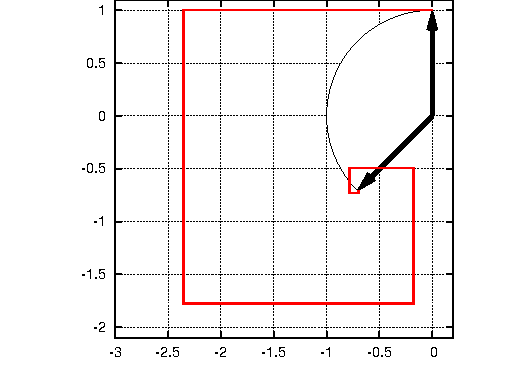
\epsfig{file=picts/C++/rotop-ulitka}
\end{center}
\caption{Пример поворота вектора $(0,1,0)$ на угол $3\pi/4$}\label{rotop:ulitka:pict} 
\end{figure}

\begin{figure}[p]
\begin{center}
\raisebox{1cm}{({\it а})}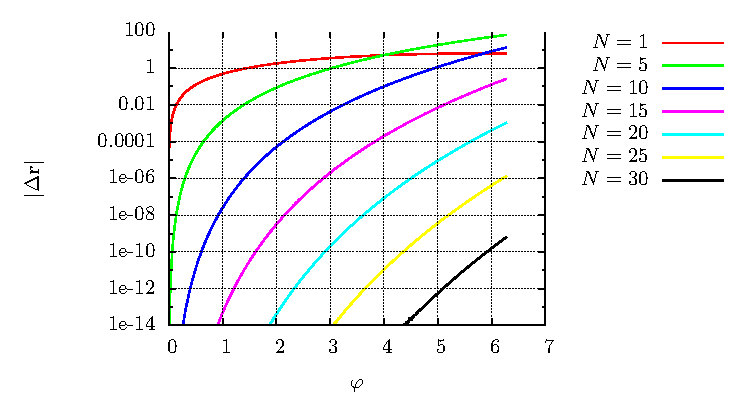
\epsfig{file=picts/C++/rotop-N-dR}
\vspace{-.5cm} 
\begin{tabular}{rl}
\raisebox{1cm}{({\it б})}\hspace{-1cm}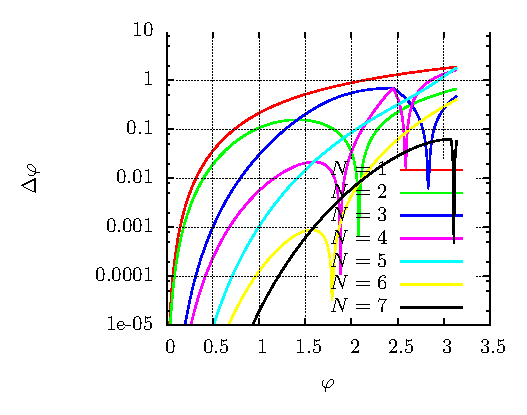
\epsfig{file=picts/C++/rotop-N-dphi} & \raisebox{1cm}{({\it в})}\hspace{-1cm}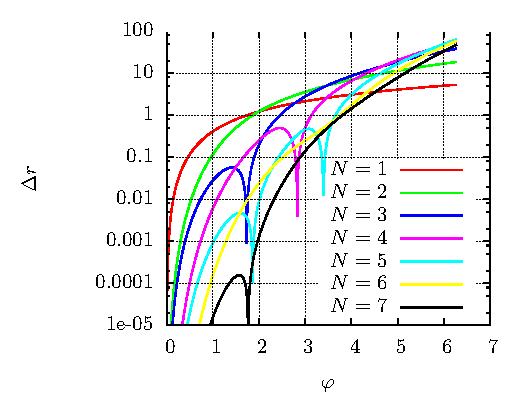
\epsfig{file=picts/C++/rotop-N-dr}\\[-.5cm]
\raisebox{1cm}{({\it г})}\hspace{-1cm}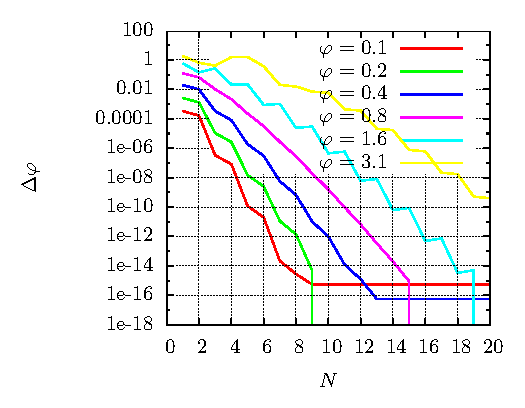
\epsfig{file=picts/C++/rotop-phi-dphi} & \raisebox{1cm}{({\it д})}\hspace{-1cm}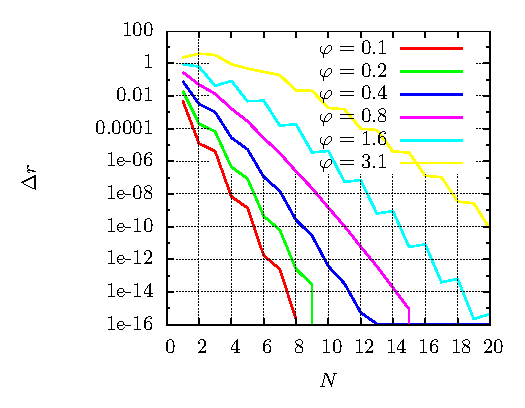
\epsfig{file=picts/C++/rotop-phi-dr}
\end{tabular}
\vspace{-.5cm} 
\end{center}
\caption{
Зависимости модуля ошибки $\vec r$ от угла поворота $\varphi$ единичного вектора $(0,1,0)$ для 
различного числа членов разложения~$N$ ({\it а}). Зависимости абсолютной ошибки по углу $\Delta\varphi$ ({\it б}) 
и модулю радиуса $\Delta r$ ({\it в}) от угла поворота $\varphi$
при использовании конечного числа членов разложения~$N$.  
Зависимости абсолютной ошибки по углу $\Delta\varphi$ ({\it г}) и радиусу $\Delta n$ ({\it д}) от числа членов разложения~$N$ 
для различных углов поворота~$\varphi$ }\label{rotop:delta:pict}
\end{figure}


Не теряя общности рассуждений, рассмотрим поворот вектора $(0,r_y,r_z)$ вокруг вертикальной оси на угол $\alpha$, 
и разложим  $\sin\alpha$ и $\cos\alpha$ в ряд в окрестностях точки $\alpha=0$:
$$
\vctr3{0}{r_y}{r_z}\rotop\vctr3{0}{0}{\alpha} = 
\vctr3{-r_y\sin\alpha}{r_y\cos\alpha}{r_z} = 
\vctr3{- r_y \sum\limits_{n=0}^\infty \frac{(-1)^n}{(2n+1)!} \alpha^{2n+1} }{
r_y\sum\limits_{n=0}^\infty \frac{(-1)^n}{(2n)!} \alpha^{2n} }{r_z} = 
\vctr3{- r_y \sum\limits_{n=0}^\infty \frac1{n!} \alpha^n \sin\frac{\pi n}2 }{
r_y\sum\limits_{n=0}^\infty \frac1{n!} \alpha^n \cos\frac{\pi n}2 }{r_z}. $$
Пусть $\a\times^n\b \equiv [...[\a \underbrace{\times \b]\times ... \b]}_n$ и $\a\times^0\b \equiv\a$. 
Рассмотрим последовательность векторных произведений:
\begin{align}
\vctr3{0}{r_y}{r_z}& \times\vctr3{0}{0}{\alpha} = \vctr3{\alpha r_y}{0}{0}, \quad 
\vctr3{0}{r_y}{r_z}\times^2\vctr3{0}{0}{\alpha} = \vctr3{0}{-\alpha^2 r_y}{0}, \quad 
\vctr3{0}{r_y}{r_z}\times^3\vctr3{0}{0}{\alpha} = \vctr3{-\alpha^3 r_y}{0}{0},  \notag\\
\vctr3{0}{r_y}{r_z}& \times^4\vctr3{0}{0}{\alpha} = \vctr3{0}{\alpha^4 r_y}{0}, \quad  ..., \quad
\vctr3{0}{r_y}{r_z}\times^n\vctr3{0}{0}{\alpha} = \vctr3{ \alpha^n r_y \sin\frac{\pi n}2}{\alpha^n r_y \cos\frac{\pi n}2}{0}.
\notag
\end{align}
Тогда, с учетом четности $\cos\alpha$ и нечетности $\sin\alpha$, поворот можно представить как
$$
\a \rotop \b = \sum\limits_{n=0}^\infty \frac1{n!}\a \times^n(-\b) = \sum\limits_{n=0}^\infty \frac{(-1)^n}{n!}\a \times^n\b.
$$


Этот же результат можно получить другим способом. Рассмотрим уравнение вида
\begin{equation}
\dot\a = -\left[ \a \times \vctr3{0}{0}{\omega} \right] \label{rotop:a:omega:eq}
\end{equation}
описывающее очевидно вращение вектора $\a$ вокруг вертикальной оси с угловой скоростью~$\omega$ против часовой стрелки (если смотреть сверху). 
Дифференцируя обе части уравнения (\ref{rotop:a:omega:eq}) по времени получаем рекуррентное соотношение для произвольной производной вектора $\a$ по времени:
$$
\frac{\partial^n\a}{\partial t^n} = -\left[ \frac{\partial^{n-1}\a}{\partial t^{n-1}} \times \vctr3{0}{0}{\omega} \right] = ... 
= (-1)^n \left[ \a \times^n \vctr3{0}{0}{\omega} \right].
$$
Пусть начальное значение вектора $\a|_{t=0}=\a_0$, тогда
$$
\a_0 \rotop \vctr3{0}{0}{\omega t} = \a(t).
$$
Разложим вектор $\a$ в ряд Тейлора в окрестности точки $t=0$:
$$
\a_0 \rotop \vctr3{0}{0}{\omega t} = \sum\limits_{n=0}^\infty \frac{t^n}{n!}\frac{\partial^n\a}{\partial t^n} = 
\sum\limits_{n=0}^\infty \frac{(-1)^n}{n!} \left[ \a \times^n \vctr3{0}{0}{\omega t} \right].
$$
Пример поворота на угол $3\pi/4$ приведен на рис.~\ref{rotop:ulitka:pict}.
Зависимости ошибок разложения приведены на рис.~\ref{rotop:delta:pict}.

Разложение оператора поворота в ряд может существенно ускорить численные схемы, использующие подобные конструкции. Так, поворот через матрицу 
(функция \verb'rotate' из модуля \verb'derart' библиотеки \verb'aivlib') занимает на процессоре {\sf Intel(R) Core(TM)2 CPU U7500} около 170 тактов,
а поворот через ряд (параметризованная по числу членов  разложения $R$ функция \verb'rotop<R>' из того же модуля) требует примерно 10 тактов 
на каждый из членов разложения.

Поскольку 
$$
\a\times^{n+2}\b = - b^2 \a\times^n\b 
$$
можно представить оператор поворота в виде суммы трех векторов
\begin{multline}
\a\rotop\b = \sum\limits_{n=0}^\infty \frac{(-1)^n}{n!} \a\times^n\b = 
\a - [\a\times\b] \sum\limits_{n=0}^\infty\frac{(-1)^n b^{2n}}{(2n+1)!} 
+\\+
\big[[\a\times\b]\times\b\big] \sum\limits_{n=0}^\infty\frac{(-1)^n b^{2n}}{(2n+2)!} 
\equiv
\a - [\a\times\b]\,\beta_1(b) - \big[\b\times[\a\times\b]\big]\, \beta_2(b)
=\\= 
\a\big(1-b^2\beta_2(b)\big) - [\a\times\b]\,\beta_1(b) + \b\,(\a\cdot\b)\,\beta_2(b),
\label{rotop:3v:rotop}
\end{multline}
где
$$
\beta_1(b) = \sum\limits_{n=0}^\infty\frac{(-1)^n b^{2n}}{(2n+1)!} = \frac{\sin b}b ,
\qquad
\beta_2(b) = \sum\limits_{n=0}^\infty\frac{(-1)^n b^{2n}}{(2n+2)!} = \frac{1-\cos b}{b^2},
$$
или
$$
\a\rotop\b = \a \cos b - [\a\times\n_b] \sin b + \n_b (\a \cdot \n_b)(1-\cos b).
$$


%\subsection{Дифференцирование оператора поворота}
Рассмотрим выражение $\partial(\a\rotop\varphi\b)/\partial\varphi$, где $\b$~вектор задающий ось вращения.
\begin{multline}
\dfdx{(\a\rotop\varphi\b)} \varphi = \dfdx{}{\varphi}
\sum\limits_{n=0}^\infty \frac{(-1)^n}{n!} \a \times^n \varphi\b = 
\sum\limits_{n=1}^\infty \frac{(-1)^n\varphi^{n-1}}{(n-1)!} \a \times^n \b = \\ =
-\left[\sum\limits_{n=1}^\infty \frac{(-1)^{n-1}}{(n-1)!} \a \times^n\varphi\b\right]\times\b = 
-(\a\rotop\varphi\b)\times\b = \b \times(\a\rotop\varphi\b).
\notag%\label{diff:rotop:eq}
\end{multline}

\endinput
%%%%%%%%%%%%%%%%%%%%%%%%%%%%%%%%%%%%%%%%%%%%%%%%%%%%%%%%%%%%%
%Аналогично, 
Рассмотрим выражение $\partial(\a(t)\rotop\varphi(t)\b)/\partial t$, где $\b$~вектор задающий ось вращения:
\begin{multline}
\dfdx{(\a(t)\rotop\varphi(t)\b)} t = \dfdx{}{t}
\sum\limits_{n=0}^\infty \frac{(-1)^n}{n!} \a(t) \times^n \varphi(t)\b = \\
= \sum\limits_{n=0}^\infty \frac{(-1)^n}{n!}\left[ \dfdx\a t \times^n \varphi \b +
 n \varphi^{n-1} \dfdx\varphi t \a \times^n \b \right] = \\ =
\dfdx\a t \rotop \varphi \b -\dfdx\varphi t \left[\sum\limits_{n=1}^\infty \frac{(-1)^{n-1}}{(n-1)!} \a \times^{n-1}\varphi\b\right]\times\b = \\
 = \dfdx\a t \rotop \varphi \b + \dfdx\varphi t \b \times(\a\rotop\varphi\b).
\label{rotop:da:dt:eq}
\end{multline}

На основе (\ref{rotop:3v:rotop}) получаем
$$
\beta_1'(b) = \frac{b\cos b-\sin b}{b^2}, \qquad \beta_2'(b) = \frac{b^2 \sin b - 2b(1-\cos b)}{b^4},
$$
откуда
\begin{multline}
\dfdx{(\a(t)\rotop\b(t))} t = 
\dot\a\big(1-b^2\beta_2(b)\big) - \a\big(2b\beta_2(b)\dot b + b^2\beta'_2(b)\dot b\big) 
-\\- [\dot\a\times\b]\,\beta_1(b) - [\a\times\dot\b]\,\beta_1(b) - [\a\times\b]\,\beta'_1(b) \dot b
+\\+ \dot\b\,(\a\cdot\b)\,\beta_2(b) + \b\,(\dot\a\cdot\b)\,\beta_2(b) + \b\,(\a\cdot\dot\b)\,\beta_2(b) +
\b\,(\a\cdot\b)\,\beta_2'(b) \dot b
=\\=
\dot\a \cos b + \a \dot b \sin b
- [\dot\a\times\b]\,\beta_1(b) - [\a\times\dot\b]\,\beta_1(b) - [\a\times\b]\,\frac{b\cos b-\sin b}{b^2} \dot b
+\\+ \dot\b\,(\a\cdot\b)\,\beta_2(b) + \b\,(\dot\a\cdot\b)\,\beta_2(b) + \b\,(\a\cdot\dot\b)\,\beta_2(b) +
\b\,(\a\cdot\b)\,\frac{b^2 \sin b - 2b(1-\cos b)}{b^4} \dot b
.
\label{rotop:da:dt:33v:eq}
\end{multline}

\begin{multline}
\dfdx{\a\rotop\b} t = \dot\a \cos b - \a\dot b \sin b 
- [\dot\a\times\n_b] \sin b - [\a\times\dot\n_b] \sin b  - [\a\times\n_b] \dot b\cos b 
+\\+ \dot\n_b (\a \cdot \n_b)(1-\cos b) + \n_b (\dot\a \cdot \n_b)(1-\cos b) + \n_b (\a \cdot \dot\n_b)(1-\cos b) 
+ \n_b (\a \cdot \n_b)\dot b \sin b 
=\\=
\dot\a \cos b - [\dot\a\times\n_b] \sin b + \n_b (\dot\a \cdot \n_b)(1-\cos b)  
-\\- 
\a\dot b \sin b - [\a\times\n_b] \dot b\cos b + \n_b (\a \cdot \n_b)\dot b \sin b 
-\\- [\a\times\dot\n_b] \sin b   
+ \dot\n_b (\a \cdot \n_b)(1-\cos b)  + \n_b (\a \cdot \dot\n_b)(1-\cos b) 
\end{multline}







\section{Операции бинарного потокового ввода/вывода --- модуль {\tt binaryio}}\label{binaryio:sec}
Модуль \verb'binaryio' перегружает операции
\begin{verbatim}
   template<typename T> inline IOstream& operator < (IOstream& S, const T& X);
   template<typename T> inline IOstream& operator > (IOstream& S,       T& X);
\end{verbatim}
как операции бинарного ввода/вывода в поток \verb'aiw::IOstream' для большинства актуальных типов \verb'T'.
Операции перегружены для встроенных типов \verb'int8_t', \verb'uint8_t', \verb'int16_t', \verb'uint16_t', \verb'int32_t', \verb'uint32_t', \verb'int64_t', \verb'uint64_t',
\verb'char', \verb'bool', \verb'float', \verb'double', типов \verb'std::complex<T>', \verb'std::string',
\verb'T[D]', \verb'std::vector<T>', \verb'std::list<T>', \verb'std::map<T1,T2>', \verb'aiw::Vec<D,T>',
и типов для которых определены публичные методы
\begin{verbatim}
    void dump(aiw::IOstream &S) const;
    void load(aiw::IOstream &S);
\end{verbatim}
Кроме того модуль предоставляет макрос
\begin{verbatim}
#define BINARYIO4POD                                                           \
    inline void dump(aiw::IOstream &S) const { S.write(this, sizeof(*this)); } \
    inline void load(aiw::IOstream &S)       { S.read(this, sizeof(*this)); }  
\end{verbatim}
вызов которого в \verb'POD'--типе объявляет методы \verb'dump/load' и автоматически перегружает операции \verb'<' и \verb'>'.

\section{Настройка пользовательских классов~--- модуль {\tt objconf}}\label{objconf:sec}
Модуль \verb'objconf' предоставляет макрос
\begin{verbatim}
    #define CONFIGURATE(ARGS...)
\end{verbatim}
который при вызове внутри пользовательского класса
\begin{verbatim}
    struct A{
        int x; double y; bool z;
        CONFIGURATE(x, y, z);
    };
\end{verbatim}
создает в классе метод
\begin{verbatim}
    template<typename ConfT>					
    void configurate(ConfT &conf, bool wmode, const char *prefix="");
\end{verbatim}
который в зависимости от значения аргумента \verb'wmode' вызывает методы
\begin{verbatim}
    conf.set(prefix+name, parametr); // wmode==true
    conf.get(prefix+name, parametr); // wmode==false
\end{verbatim}
для каждого из полей класса, перечисленных в аргументах макроса \verb'CONFIGURATE'.
Аргумент \verb'prefix' позволяет добавить префикс к именам всех полей при чтении/записи.

Созданный метод \verb'configurate(...)' может использоваться при чтении/записи конфигурационных файлов (раздел~\ref{configfile:sec}),
записи состояния объекта в формате \verb'pickle' (раздел~\ref{pickle:sec}) и т.д.

\section{Чтение и запись конфигурационных файлов~--- модуль {\tt configfile}}\label{configfile:sec}
Модуль \verb'configfile' состоит из заголовчного файла \verb'configfile' и файла \verb'src/configfile.cpp',
и предоставляет средства для чтения/записи конфигурационных файлов в текстовом формате
\begin{verbatim}
    # комментарий
    имя_параметра=значение параметра
\end{verbatim}
для каждого параметра может использоваться {\bf только одна} строка. 

Модуль определяет функции чтения/записи для различных типов из потоков ввода/вывода \verb'std::iostream'
\begin{verbatim}
    template <typename T> void printf_obj(std::ostream &S, const T &X){ S<<X; }
    template <typename T> void scanf_obj(std::istream &S, T &X){ S>>X; }
\end{verbatim}
которые могут быть перегружены специальным образом для отдельных типов
\begin{verbatim}
    void printf_obj(std::ostream &S, bool X);
    void scanf_obj(std::istream &S, bool &X);

    template <typename T> void printf_obj(std::ostream &S, const std::complex<T> &X);
    template <typename T> void scanf_obj(std::istream &S, std::complex<T> &X);

    void scanf_obj(std::istream &S, std::string &X);
\end{verbatim}
для типа \verb'bool' допустимыми являются значения в конфигурацинном файле
\begin{verbatim}
  Y y YES Yes yes ON  On  on  TRUE  True  true  V v 1
  N n NO  No  no  OFF Off off FALSE False false X x 0
\end{verbatim}
Для типа \verb'std::complex' используется формат \verb'Python' $x\pm y$\verb'j'.

Для типа \verb'std::string' при чтении из конфигурационного файла используется строка после знака \verb'=' с отброшенными с конца и начала символами
пробела, \verb'\t' и \verb'\r' (аналог вызывова функции \verb'str.strip()' языка \verb'Python').

Непосредственно для чтения/записи конфигурационного файла используется класс
\begin{verbatim}
    class ConfigFile{
    public:
        int no_key_act = 2; // 0 - ignore, 1 - warning, 2 - exception
    #ifndef SWIG
        // получает значение параметра par с именем key из другого объекта 
        //        для записи в конфигурационный файл
        template <typename T> 
        void get(const std::string &key, const T &par);
        // устанавливает значение параметра par с именем key в другом объекта 
        //        на основе конфигурационного файла
        template <typename T> 
        void set(const std::string &key, T &par);

        void load(std::istream &&fin);
        void dump(std::ostream &&fout) const;
        void load(std::istream &fin);
        void dump(std::ostream &fout);
    #endif //SWIG		
        void load(const char *path);
        void dump(const char *path) const;
        void clear();
    };
\end{verbatim}

При чтении конфигурациооного файла для экземпляра класса \verb'ConfigFile' вызывается один из методов \verb'load', затем экземпляр класса
передается первым аргументов в методы \verb'configurate' настраиваемых пользовательских объектов, см. раздел~\ref{objconf:sec}.
Поле \verb'no_key_act' управляет реакцией на отсутствие какого либо параметра в конфигурационном файле: \verb'0'~--- игнорировать,
\verb'1'~-- выдать предупреждение, \verb'2'~--- сгенерировать исключение.

При записи конфигурациооного файла экземпляра класса \verb'ConfigFile'
передается первым аргументов в методы \verb'configurate' настраиваемых пользовательских объектов, см. раздел~\ref{objconf:sec},
затем для него необходимов вызвать один из методов~\verb'dump'.




% сфера
% инстацирование в питон - размазать по предыдыщуим модулям?

\end{document}

\chapter{Средства визуализации}
%3.1 gplt
%3.2 arr2D
%3.3 arr3D
%3.4 сфера
%3.5 вьювер для поверхностей
%3.6 вьювер для магнетиков

\chapter{RACS}

\chapter{Система кодогенерации SYMBALG}

\chapter{Дополнительные модули для питона}

\chapter{Алгоритмы}
\subsection{Построение изолиний}
\subsection{Интерполяция}

\end{document}
%\input{aivlib/installation}

\chapter{Ядро библиотеки}
\section{Введение}
\section{Введение}

Интерфейс приложения численного моделирования должен позволять
легко изменять параметры задачи (число которых иногда доходит до сотен или даже тысяч),
выбирать тот или иной алгоритм (в том числе разлиные варианты начальных и граничных условий),
обеспечивать анализ и визуализацию
результатов. Практика показала, что для сложных задач оптимальным
являеться не оконный интерфейс, а интерфейс командной
строки. Фактически речь идет о использовании собственного (или уже
существующего) высокоуровневого интерпретируемого языка,
адаптированного к специфике задачи.

При проведении массовых расчетов (например при анализе зависимости поведения устройства от 
нескольких параметров и построении фазовых диаграмм) требуется механизм, обеспечивающий
многократный автоматический запуск приложения с меняющимися заданным образом параметрами, 
желательно с контролем распределения ресурсов в рамках локальной сети или на кластере.

Для каждого расчета полученные зависимости должны сопровождаться
информацией о использованных параметрах расчета и алгоритмах. Если для
сохранения параметров существует большое количество методик и
библиотек, то сохранение алгоритмов является проблемой, и единственным
приемлемым решением на сегодняшний день является сохранение исходного
кода приложения.

Для анализа результатов необходим многопараметрический поиск по
проведенным расчетам, для чего результаты расчетов должны храниться
специальным, упорядоченным образом. Необходимо обеспечить возможность
поиска по версиям исходного кода. Эту проблему можно решать в ручную,
например размещая результаты расчетов на хорошо структурированном дереве
каталогов~--- однако такой подход требует строгой внутренней культуры пользователя, и
усложняется тем, что в процессе расчетов критерии упорядоченности могут
расширятся и изменяться кардинальным образом.   

При массовых расчетах аккуратное решение вышеописанных проблем может отнимать значительное время и силы. 
В разных рабочих группах
разработаны собственные библиотеки, позволяющие упростить процесс
написания окружения, но единый подход до сих пор не выработан.

Описанная в данной главе система {\tt RACS} ({\tt Results \& Algorithms Control System}~--- система контроля
результатов и алгоритмов) обеспечивает:
\begin{itemize}
\item задание параметров расчетов при запуске для приложений на языках \verb'Python' и \verb'C++';
\item автоматическое сохранение параметров и исходных кодов расчетов;
\item пакетный запуск расчетов (циклы по значениям параметров) и балансировка загрузки, как на локальных машинах так и на кластерах под \verb'MPI';
\item работа с контрольными точками для приложений \verb'C++', в том числе кластерах под \verb'MPI' ({\it в разработке});
\item развитые средства для многопараметрического поиска, анализа и обработки результатов.
\end{itemize}

При разработке \verb'RACS' делались следующие акценты:
\begin{itemize}
\item простота подключения (требуется минимальная модификация отлаженного кода);
\item лаконичный и интуитивно понятный синтаксис при запуске расчетов;
\item возможность обработки результатов средствами операционной системы и сторонними утилитами без потери целостности данных;
\item интеграция с другими утилитами~--- вывод данных в формате \verb'gnuplot' с заголовками \verb'gplt',
  чтение метаинформации о расчетах другими утилитами.
\end{itemize}


Даже для низкоквалифицированного
пользователя  {\tt RACS} автоматически обеспечивает необходимый минимум
<<культуры>> проведения расчетов (сохранение исходных кодов  и
параметров).
В результате пользователь имеет
возможность полностью сконцентрироваться на работе непосредственно  над задачей.

\verb'RACS' написан на языке \verb'Python' и ориентирован в первую очередь
на приложения написанные на
языках \verb'C++' (высокопроизводительное вычислительное ядро) и \verb'Python' (верхний управляющий слой приложения и
интерфейсные части), связанные при помощи утилиты \verb'SWIG'~\cite{SWIG}.

К настоящему моменту (первые версии появились в 2003 году, первая публикация \cite{racs:2007} в 2007 году) 
{\tt RACS} хорошо зарекомендовал себя при организации массовых расчетов в различных областях~--- сейсмике,
моделировании разработки керогеносодержащих месторождений с учетом внутрипластового горения,
моделировании магнитных систем и разработке устройств спинтроники, %физике плазмы,
газодинамике горения, изучении резонансных свойств нелинейных систем и т.д.
%Тем не менее, в процессе эксплуатации был обнаружен ряд недостатков, требующих существенной доработки системы.

\endinput

Целый ряд задач численного моделирования требует проведения больших объемов
однотипных серий расчетов~--- расчеты в серии независимы, и отличаются
лишь значением одного или нескольких параметров, и именно в этом в этом случае
{\tt RACS} оказывается наиболее эффективен. 
Кроме поиска в результатах расчетов, запущенный в клиент--серверном режиме {\tt RACS} обеспечивает автоматический
запуск расчетов на нескольких компьютерах в рамках кластера или локальной сети с разнородными версиями 
операционной системы.
Инструментальные средства {\tt Python} и {\tt RACS} позволяют реализовывать
консервацию и восстановление расчета для продолжения.


Изначально {\tt RACS} был построен по асинхронной схеме, без центрального сервера (такая архитектура
представлялась более надежной). Появившийся со временем сервер 
занимался лишь даигностикой и сбором статистики загруженности ресурсов.
Практика показала, что при интенсивных разнородных расчетах в рамках локальной сети или кластера 
такая архитектура не позволяет 
должным образом распределять ресурсы, что приводит к эпизодическим конфликтам. 

Интерфейс подключения {\tt RACS} к приложениям численного моделирования так же может быть существенно улучшен.
В настоящий момент подключение {\tt RACS} к уже готовому коду требует рутинной переработки кода, что неизбежно приводит
к ошибкам. Представляется возможным организовать подключение с минимальными изменениями отлаженного ранее кода.

С другой стороны, за время эксплуатации был накоплен большой опыт по организации массовых расчетов и 
постобработке результатов моделирования,  сформулированна соответствующая идеология. Разработанные подходы должны быть 
особенно эффективны при решении инженерных задач, требующих проведения больших объемов однотипных расчетов и комплексного 
анализа их результатов для выбора
оптимальной конфигурации устройства.

\section{Общие модули}
Для всех классов и функций библиотеки {\tt aivlib} необходимы потоки ввода/вывода, индексы и вектора~--- это
то <<основание>>, на котором строятся все остальные библиотечные классы и функции.
\input{aivlib/mystream}
\input{../tests/mystream}

\input{aivlib/IndxVctr}
\input{../tests/IndxVctr}

\input{aivlib/dekart}

\section{Контейнеры}
\input{aivlib/array}
\small
\input{../tests/Arr2D}
\input{../tests/Arr3D}
\normalsize
\input{aivlib/sphere}
\input{../tests/sphereT}


\section{Классы и функции для построения изображений}
%\input{aivlib/images}
%\input{tests/images}
\begin{center}
\framebox{************* раздел находится в разработке ****************}
\end{center}

\section{Утилиты командной строки}
\input{aivlib/shellutils}
\input{aivlib/viewers}


\chapter{Система контроля результатов и алгоритмов RACS}
\section{Введение}

Интерфейс приложения численного моделирования должен позволять
легко изменять параметры задачи (число которых иногда доходит до сотен или даже тысяч),
выбирать тот или иной алгоритм (в том числе разлиные варианты начальных и граничных условий),
обеспечивать анализ и визуализацию
результатов. Практика показала, что для сложных задач оптимальным
являеться не оконный интерфейс, а интерфейс командной
строки. Фактически речь идет о использовании собственного (или уже
существующего) высокоуровневого интерпретируемого языка,
адаптированного к специфике задачи.

При проведении массовых расчетов (например при анализе зависимости поведения устройства от 
нескольких параметров и построении фазовых диаграмм) требуется механизм, обеспечивающий
многократный автоматический запуск приложения с меняющимися заданным образом параметрами, 
желательно с контролем распределения ресурсов в рамках локальной сети или на кластере.

Для каждого расчета полученные зависимости должны сопровождаться
информацией о использованных параметрах расчета и алгоритмах. Если для
сохранения параметров существует большое количество методик и
библиотек, то сохранение алгоритмов является проблемой, и единственным
приемлемым решением на сегодняшний день является сохранение исходного
кода приложения.

Для анализа результатов необходим многопараметрический поиск по
проведенным расчетам, для чего результаты расчетов должны храниться
специальным, упорядоченным образом. Необходимо обеспечить возможность
поиска по версиям исходного кода. Эту проблему можно решать в ручную,
например размещая результаты расчетов на хорошо структурированном дереве
каталогов~--- однако такой подход требует строгой внутренней культуры пользователя, и
усложняется тем, что в процессе расчетов критерии упорядоченности могут
расширятся и изменяться кардинальным образом.   

При массовых расчетах аккуратное решение вышеописанных проблем может отнимать значительное время и силы. 
В разных рабочих группах
разработаны собственные библиотеки, позволяющие упростить процесс
написания окружения, но единый подход до сих пор не выработан.

Описанная в данной главе система {\tt RACS} ({\tt Results \& Algorithms Control System}~--- система контроля
результатов и алгоритмов) обеспечивает:
\begin{itemize}
\item задание параметров расчетов при запуске для приложений на языках \verb'Python' и \verb'C++';
\item автоматическое сохранение параметров и исходных кодов расчетов;
\item пакетный запуск расчетов (циклы по значениям параметров) и балансировка загрузки, как на локальных машинах так и на кластерах под \verb'MPI';
\item работа с контрольными точками для приложений \verb'C++', в том числе кластерах под \verb'MPI' ({\it в разработке});
\item развитые средства для многопараметрического поиска, анализа и обработки результатов.
\end{itemize}

При разработке \verb'RACS' делались следующие акценты:
\begin{itemize}
\item простота подключения (требуется минимальная модификация отлаженного кода);
\item лаконичный и интуитивно понятный синтаксис при запуске расчетов;
\item возможность обработки результатов средствами операционной системы и сторонними утилитами без потери целостности данных;
\item интеграция с другими утилитами~--- вывод данных в формате \verb'gnuplot' с заголовками \verb'gplt',
  чтение метаинформации о расчетах другими утилитами.
\end{itemize}


Даже для низкоквалифицированного
пользователя  {\tt RACS} автоматически обеспечивает необходимый минимум
<<культуры>> проведения расчетов (сохранение исходных кодов  и
параметров).
В результате пользователь имеет
возможность полностью сконцентрироваться на работе непосредственно  над задачей.

\verb'RACS' написан на языке \verb'Python' и ориентирован в первую очередь
на приложения написанные на
языках \verb'C++' (высокопроизводительное вычислительное ядро) и \verb'Python' (верхний управляющий слой приложения и
интерфейсные части), связанные при помощи утилиты \verb'SWIG'~\cite{SWIG}.

К настоящему моменту (первые версии появились в 2003 году, первая публикация \cite{racs:2007} в 2007 году) 
{\tt RACS} хорошо зарекомендовал себя при организации массовых расчетов в различных областях~--- сейсмике,
моделировании разработки керогеносодержащих месторождений с учетом внутрипластового горения,
моделировании магнитных систем и разработке устройств спинтроники, %физике плазмы,
газодинамике горения, изучении резонансных свойств нелинейных систем и т.д.
%Тем не менее, в процессе эксплуатации был обнаружен ряд недостатков, требующих существенной доработки системы.

\endinput

Целый ряд задач численного моделирования требует проведения больших объемов
однотипных серий расчетов~--- расчеты в серии независимы, и отличаются
лишь значением одного или нескольких параметров, и именно в этом в этом случае
{\tt RACS} оказывается наиболее эффективен. 
Кроме поиска в результатах расчетов, запущенный в клиент--серверном режиме {\tt RACS} обеспечивает автоматический
запуск расчетов на нескольких компьютерах в рамках кластера или локальной сети с разнородными версиями 
операционной системы.
Инструментальные средства {\tt Python} и {\tt RACS} позволяют реализовывать
консервацию и восстановление расчета для продолжения.


Изначально {\tt RACS} был построен по асинхронной схеме, без центрального сервера (такая архитектура
представлялась более надежной). Появившийся со временем сервер 
занимался лишь даигностикой и сбором статистики загруженности ресурсов.
Практика показала, что при интенсивных разнородных расчетах в рамках локальной сети или кластера 
такая архитектура не позволяет 
должным образом распределять ресурсы, что приводит к эпизодическим конфликтам. 

Интерфейс подключения {\tt RACS} к приложениям численного моделирования так же может быть существенно улучшен.
В настоящий момент подключение {\tt RACS} к уже готовому коду требует рутинной переработки кода, что неизбежно приводит
к ошибкам. Представляется возможным организовать подключение с минимальными изменениями отлаженного ранее кода.

С другой стороны, за время эксплуатации был накоплен большой опыт по организации массовых расчетов и 
постобработке результатов моделирования,  сформулированна соответствующая идеология. Разработанные подходы должны быть 
особенно эффективны при решении инженерных задач, требующих проведения больших объемов однотипных расчетов и комплексного 
анализа их результатов для выбора
оптимальной конфигурации устройства.

\input{racs/formalism}
\input{racs/general}
\input{racs/pickle_db}
\section{Анализ и обработка результатов~--- утилита командной строки {\tt racs}}



\input{racs/sh_utils}
\input{racs/grid}

\section{Модуль {\sf mixt.py} --- набор служебных функций и классов}
Модуль {\sf mixt.py} содержит ряд функций, использующихся остальными модулями
библиотеки {\sf raclib}.

\subsection{Различные системные функции}
Функция \verb'except_report( stderr=sys.stderr )' выводит отчет о последней
ошибке (возбужденном исключении) включая стек в файловый объект {\sf stderr} и возвращает
список строк отчета об ошибке виде результата. 

Функция \verb'get_checksums( Lf )' вовращает список контрольных сумм для
файлов из списка {\sf Lf}, контрольные суммы считаются при помощи утилиты {\sf
md5sum}.

Функции \verb'time2string( t, precision=3 )' и \verb'string2time( S )'
преобразуют число секунд {\sf t} в строку {\sf S} вида \verb|'hours:mm:sec'| и
обратно. Число знаков после десятичной точки при отображении секунд задается
аргументом {\sf precision}. Функции устаревшие, рекомендуется использовать класс {\sf mytime.Time}.

Функции \verb'date2string( d )' и \verb'string2date( S )'
преобразуют дату {\sf d} (число секунд  с начала эпохи {\sf Unix}) в строку {\sf S} вида \verb|'YYYY:MM:DD-hh:mm:sec'| и
обратно. Функции устаревшие, рекомендуется использовать класс {\sf mytime.Date}.

Функция \verb'size2string( sz )' преобразует размер {\sf sz} в байтах в строку
вида '$XXX${\sf K}' либо '$XXX.X${\sf M}' либо '$XXX.X${\sf G}' либо '$XXX.X${\sf T}'.

Функция \verb'GetLogin()' возвращает имя пользователя, пытаясь сначала вызвать
функцию \verb'os.getlogin()' а в случае ошибки возвращает занчение переменной
окружения {\sf USER}


Функция \verb'compare( name, patterns )' проверяет  при помощи функции {\sf
  fnmatch.fnmatch(...)} \cite{GVR} соответствует ли строка {\sf name} одному из
шаблонов в списке {\sf patterns}. Шаблоны могут иметь стандартный вид {\sf
  shell}, т.е. включать символы \verb|'*'|, \verb|'?'| и т.д. Если найдено соотвествие
хотя бы одному из шаблонов  возвращается {\sf True}, иначе возвращается {\sf False}.

Функция \verb'str_len( S )' возвращает длину строки \verb'S' в символах (при печати),
учитывая что символы {\sf utf-8} занимают два байта в памяти и один символ на
печати.

Функция \verb'get_tty_width()' возвращает ширину текущего терминала, запуская
в {\sf shell} команду \verb'stty size' и анализируя ее вывод.

Функция
\verb'table2strlist( LL, pattern=None, s_line=1, s_empty=2, s_bound=1, max_len=None )'
возвращает список форматированных строк (без символа конца строки
\verb|'\n'|). Аргумент \verb'LL' это таблица (список списков), для включения разделителя
(горизонтальной линии) необходимо вставить в \verb'LL' значение {\sf
  None}, все остальные элементы \verb'LL' должны быть списками или кортежами
одинаковой длины и содержать величины, которые при выводе будут
преобразовываться к строке при помощи функции {\sf str()}. Аргумент
\verb'pattern' задает паттерн аналогичный заголовку таблиц \LaTeX, т.е. может
содержать символы \verb|'r'|, \verb|'c'|, \verb|'l'| для обозначения
выравнивания содержимого колонки или символ \verb-'|'- для задания
вертикальной линии между колонками. Аргументы \verb's_line', \verb's_empty',
\verb's_bound' задают число пробелоов между текстом и вертикальными
разделительными линиями, между колонками без вертикальных разделительных линия
линий и между колонками и краями (если по краям нет линий). Аргумент
\verb'max_len' задает максимальную длину строк в выводимом списке (по
умолчанию без ограничений), лишние символы отбрасываются.



\subsection{Создание уникальных директорий расчета}
Функция  \verb'make_unique_path( base_path, num=3 )' генерирует уникальное имя
директории, добавляя к \verb'base_path' необходимое минимальное число
дополненное с начала нулями до длины {\sf num}. Например, если в директории
\verb'mypath/' есть поддиректория (или файл) с именем \verb'a023' то вызов 
\verb|make_unique_path( 'mypath/a' )| вернет строку \verb|'mypath/a024'|.

Функция \verb'close_path( p )' добавляет в конец пути {\sf p} символ
\verb|'/'| если {\sf p} не заканчивается этим символом.

Функция \verb'make_path( repository )' создает уникальную директорию в
репозитории \verb"repository" (в том числе и сам репозиторий при необходимости) и возвращает путь к ней.
Название директории формируется из
года, номера недели, дня недели и некоторого трехзначного порядкового номера
уникального для данной даты~--- таким образом расчеты внутри
репозитория автоматически
упорядочиваются по дате (например {\sf
  c07\_00\_1005}~--- пятый расчет проведенный первого января 2007
года). 
В рабочем каталоге (из которого была вызвана функция \verb'make_path') на директорию создается
символическая ссылка \verb|'_'| (одиночный символ подчеркивания).


\subsection{Класс {\sf progressbar} для интерактивного отображения степени
  выполнения вычислений}
Класс {\sf progressbar} обеспечивает интерактивное отображение степени
выполнения вычислений в стандатрном выводе или в стандартном потоке ошибок,
автоматически экстраполируя время завершения вычислений. Конструктор класса
принимает единственный аргумент~--- стандартный поток вывода {\sf sys.stdout} (по умолчанию)
или стандартный поток ошибок {\sf sys.stderr}. 

Класс имеет следующие методы:
\begin{itemize}
\item \verb'clean()' --- сбрасывает состояние объекта для отображения степени
  выполнения нового процесса;
\item \verb|out( progress, prompt='' )| --- отображает степень выполнения {\sf
progress} (число от нуля до единицы) и выводит некоторую дополнительную
  информацию {\sf prompt};
\item \verb|close( prompt='', result='OK' )| --- завершает отображение степени
  выполнения,  выводит  некоторую дополнительную
  информацию {\sf prompt} и результат выполнения {\sf result}. 
\end{itemize}

Отображение производится в виде строки 
\begin{verbatim}
<PROMPT> <RUNTIME> from <TOTALTIME> [###          ]
\end{verbatim}
где \verb'<RUNTIME>' --- время прошедшее с начала выполнения отображаемого
процесса, \verb'<TOTALTIME>'~--- оценка общего времени выполнения процесса
(может быть весьма неточной), строка \verb|'[###          ]'| отображает степень
выполнения. Общая длина строки всегда равняется ширине терминала (определяется
при помощи функции \verb'get_tty_width()'), поэтому не следует использовать слишком
длинные варианты {\sf prompt}.

Если поток, в который экземпляр класса {\tt progressbar} производит вывод, был перенаправлен в файл 
(или изначально являлся обычным файлом и не был связан с терминалом), вывод производится только методом {\tt close()}.

\subsection{Класс {\sf reg} --- задание интервалов значений для сравнения}

Модуль содержит определение глобальных величин
\begin{verbatim}
    inf, nan = float('inf'), float('nan')
\end{verbatim}
для операций сравнения.

Класс {\sf reg} предназначен для задания областей (интервалов) значений
произвольного типа для сравнения. Для класса определены следующие операторы:
\begin{center}
\begin{tabular}{rclcrcl}
\verb'reg(a,b)' &$\to$& $[a,b]$ &\rule{1cm}{0pt}&
\verb'x in reg(a,b)' &$\to$& $x\in [a,b]$ \\
\verb'reg(a,b) < x' &$\to$& $x>b$ && 
\verb'reg(a,b) <= x' &$\to$& $x\ge b$ \\
\verb'x < reg(a,b)' &$\to$& $x<a$ && 
\verb'x <= reg(a,b)' &$\to$& $x\le a$ \\
\verb'reg(a,b) > x' &$\to$& $x<a$ &&
\verb'reg(a,b) >= x' &$\to$& $x\le a$ \\
\verb'x > reg(a,b)' &$\to$& $x>b$ &&
\verb'x >= reg(a,b)' &$\to$& $x\ge b$ \\
\verb'reg(a,b) == x' &$\to$& $x \in [a,b]$ &&
\verb'reg(a,b) != x' &$\to$& $x \notin [a,b] $ \\
\verb'x == reg(a,b)' &$\to$& $x \in [a,b]$ &&
\verb'x != reg(a,b)' &$\to$& $x \notin [a,b] $ \\
\verb'reg(a,b) + X' &$\to$& $[a,b] \cup X$ &&
\verb'X + reg(a,b)' &$\to$& $X \cup [a,b]$ \\
\verb'reg(a,b)*x' &$\to$& $[ax,bx]$ &&
\verb'x*reg(a,b)' &$\to$& $[xa,xb]$ \\
\verb'reg(a,b)/x' &$\to$& $[a/x,b/x]$ &&
\verb'-reg(a,b)' &$\to$& $[b,a]$ \\
\end{tabular}
\end{center}
где $a, b, x$~--- некоторые значения допускающие сравнения, $X$~--- экземпляр
класса {\sf reg} или некоторое значение допускающее сравнение. Оператор суммы
возвращает кортеж из региона и добавленного значения, поэтому операторы
сравнения для него не работают, но работает оператор {\sf 'in'}.

\input{racs/mytime}
\input{racs/examples}


\chapter{Различные пакеты и утилиты}
\section{Модуль {\tt bindopt}~--- разбор аргументов командной строки в приложениях
{\tt Python}}\label{igl:sec}
\input{other/bindopt}

\section{Модуль {\tt myTkinter} --- упрощенное создание оконных интерфейсов}
\input{other/myTkinter}

\section{Утилита {\tt convolve}}\label{convolve:sec}
\input{other/convolve}
\clearpage

\section{Утилита {\tt gplt} --- упрощенное создание графиков типографского качества}\label{gplt:sec}
\input{other/gplt}

\chapter{Система кодогенерации SYMBALG}
%\input{symbalg/symbalg}
\begin{center}
\framebox{************* раздел находится в разработке ****************}
\end{center}

\begin{thebibliography}{99}
\bibitem{GVR}  Г. Россум, Ф.Л.Дж. Дрейк, Д.С. Откидач. <<Язык программирования
  {\tt Python}>>. 2001~--- 454C.
\bibitem{ML} Марк Лутц. Программирование на {\tt Python}. С-Пб.:
  <<Символ>>. 2002~--- 1135C. 
\bibitem{MAKE} Ричард Столлман, Роланд МакГрат. <<{\tt GNU Make}. Программа
  управления компиляцией>> 1995.
\bibitem{aiv:cpp2py} \href{http://a-iv.ry/pyart/cpp2py.pdf}
{А.В. Иванов <<Импорт {\tt С++} кода  в {\tt Python} при помощи пакета {\bfseries\tt SWIG}>>}
\bibitem{bash:conspect} 
\href{http://www.linux.org.ru/books/bash-conspect.html}{Григорий Строкин <<BASH конспект>> 1997.}
\bibitem{bash:scripting} Mendel Cooper <<Advanced Bash-Scripting Guide>>, перевод: Андрей
  Киселев
  \href{http://www.opennet.ru/docs/RUS/bash\_scripting\_guide/}{<<Искусство программирования на языке сценариев командной оболочки>>}
\end{thebibliography}

%\input{../tests/indexD}

\end{document}
%%%%%%%%%%%%%%%%%%%%%%%%%%%%%%%%%%%%%%%%%%%%%%%%%%%%%
